\section{多元统计分析部分}\label{SecMultivariateStatisticalAnalysis}
\begin{center}
    Instructor: Dong Li \& Tianying Wang
\end{center}
\subsection{Multivariate Data}
    In this section, we consider a \textbf{Multivariate Statistic Model}. Sample comes from $p$ dimension multivariate population $f(x_1,x_2,\ldots,x_p)$.

    \textbf{Notation }: In this section, we still denote random variable in upper case and observed value in lower case, specially express random vector in bold font. \textbf{But} in this section we usually omit the vector symbol $ \vec{\cdot} \,\,$. e.g.
    random vector with $ n $ \textbf{variable }is denoted as $\mathbf{X}=(X_{\cdot 1},X_{\cdot 2},\ldots ,X_{\cdot p})$; sample of size $ n $ from the multivariate population is a $ n\times p $ matrix $ \{x_{ij}\} $, each sample item (a row in sample matrix) is denoted as $ x_i' $ or $ x_i^T $.\footnote{Here sample item (or sample case) $x_i=[x_{i1},x_{i2},\ldots,x_{ip}]^T$ is a column vector.} 
    % In this section we use the upper case $ X_i $ means that it's a vector (not necessarily means an r.v.).
    %\footnote{In previous section, a multivariate r.v. is denoted $\vec{X}=(X_1,X_2,\ldots,X_p) $, and sample item is $ \vec{X_i}=(X_{i1},X_{i2},\ldots,X_{ip})  $}


\subsubsection{Matrix Representation}


    \begin{itemize}[topsep=0pt,itemsep=1pt]
        \item \hyperlink{RandomVariableRepresentation}{Random Variable Representation}
        \item \hyperlink{SampleRepresentation}{Sample Representation}
        \item \hyperlink{StatisticsRepresentation}{Statistics Representation}
        \item \hyperlink{SampleStatisticsProperties}{Sample Statistics Properties}
    \end{itemize}
    



\begin{point}
    \hypertarget{RandomVariableRepresentation}{Random Variable Representation}:
\end{point}
    \begin{itemize}[topsep=6pt,itemsep=4pt]
        \item Random Matrix: Definition and basic properties of r.v. see \autoref{SectionPropertiesOfRandomVariableAndVector}. Now extend the definition to matrix $ X=\{X_{ij}\} $. 
    
    \begin{equation}
        X=\{X_{ij}\}=\begin{bmatrix}
        X_{11}&X_{12}&\ldots&X_{1p}\\
        X_{21}&X_{22}&\ldots&X_{2p}\\
        \vdots&\vdots&\ddots&\vdots\\
        X_{1n}&X_{n2}&\ldots&X_{np}\\
        \end{bmatrix} 
    \end{equation}

    And we can further define $ \mathbb{E}(X)=\{\mathbb{E}(X_{ij})\} $.
    For any const matrix $ A,B $ we have
    \begin{equation}
        \mathbb{E}(AXB)=A\mathbb{E}(X)B 
    \end{equation}

    \item Random Vector\index{r.v. (Random Variable or Random Vector)}: For a $ p\times 1 $ random vector $ \vec{X}=(X_{1},X_{2},\ldots,X_{p})^T  $, denote (Marginal) expectation and variance, and covariance, correlation coefficient between $ X_i,X_j $ as follows:
    \begin{align*}
        \mu_i&=\mathbb{E}(X_i)\\
        \sigma _{ii}&=\sigma_i ^2=\mathbb{E}(X_i-\mu_i)^2\\
        \sigma_{ij}&=\mathbb{E}[(X_i-\mu_i)(X_j-\mu_j)]\\
        \rho _{ij}&=\dfrac{\sigma _{ij}}{\sqrt{\sigma _{ii}}\sqrt{\sigma _{jj}}}
    \end{align*}
    
    and we have covariance matrix (as defined in \autoref{SubSubSectionCovarianceAndCorrelation}, \autoref{covariancematrix})
    \begin{equation}
        \Sigma =\mathbb{E}[(X-\mu)(X-\mu)^T] =
        \begin{bmatrix}
        \sigma _{11}&\sigma _{12}&\ldots&\sigma _{1p}\\
        \sigma _{21}&\sigma _{22}&\ldots&\sigma _{2p}\\
        \vdots&\vdots&\ddots&\vdots\\
        \sigma _{1p}&\sigma _{p2}&\ldots&\sigma _{pp}\\
        \end{bmatrix}
    \end{equation}

    and Standard Deviation Matrix
    \begin{equation}\label{EqaStandardDeviationMatrix}
        V^{1/2}=diag\{\sqrt{\sigma _{ii}}\} 
    \end{equation}

    Based on $ \vec{X}=(X_{1},X_{2},\ldots,X_{p})  $, consider the linear combination:$ Y=c'X=c_1X_1+c_2X_2+\ldots c_pX_p $
    \begin{align*}
        \mathbb{E}(y)=c'\mu\qquad var(Y)=c'\Sigma c
    \end{align*}

    and $ Z_i=\sum_{j=1}^p c_{ij}X_j $ (i.e. $ Z=CX $):
    \begin{equation}
        \mu_Z=\mathbb{E}(Z)= C\mu_X\qquad \Sigma _Z=C\Sigma _XC^T
    \end{equation}
    
    
    
    

    and Correlation Matrix\footnote{Here the correlation matrix is the matrix of Pearson's Correlation Coefficients. Another frequently use correlation matrix called Cross Correlation Matrix is\index{Correlation Matrix@(Cross) Correlation Matrix} 
    \begin{align*}
            \mathrm{cross}(X,Y)= \mathbb{E}\left[ X'Y \right]
    \end{align*}

    and correlation matrix with $ Y=X $:
    \begin{align*}
        \mathrm{cross}(X,X)=  \mathbb{E}\left[ X'X\right]
    \end{align*}
    }
    \index{Correlation Matrix@(Pearson's) Correlation Matrix}
    \begin{equation}
        \rho =\begin{bmatrix}
        \rho _{11}&\rho _{12}&\ldots&\rho _{1p}\\
        \rho _{21}&\rho _{22}&\ldots&\rho _{2p}\\
        \vdots&\vdots&\ddots&\vdots\\
        \rho _{1p}&\rho _{p2}&\ldots&\rho _{pp}\\
        \end{bmatrix} 
        =V^{-1/2}\Sigma V^{-1/2}
    \end{equation}
    
    
    \end{itemize}
    
        
\begin{point}
    \hypertarget{SampleRepresentation}{Sample Representation}:
\end{point}
    
    Sample of $n$ items from population characterized by $ p $ variables
    % \begin{table}[H]
    %     \centering
    %     \begin{tabular}{|c|cccccc|}
    %         \hline
    %         \diagbox{Item}{Variable}&Variable 1&Variable 2&$\ldots$&Variable $j$&$\ldots$&Variable $p$\\
    %         \hline
    %         Item 1&$ x_{11} $&$ x_{12} $&$ \ldots $&$ x_{1j} $&$ \ldots $&$ x_{1p} $\\
    %         Item 1&$ x_{21} $&$ x_{22} $&$ \ldots $&$ x_{2j} $&$ \ldots $&$ x_{2p} $\\
    %         $\vdots$&$\vdots$&$\vdots$&$ \ddots $&$\vdots$&$ \ddots $&$\vdots$\\
    %         Item $j$&$ x_{i1} $&$ x_{i2} $&$ \ldots $&$ x_{ij} $&$ \ldots $&$ x_{ip} $\\
    %         $\vdots$&$\vdots$&$\vdots$&$ \ddots $&$\vdots$&$ \ddots $&$\vdots$\\            
    %         Item $n$&$ x_{n1} $&$ x_{n2} $&$ \ldots $&$ x_{nj} $&$ \ldots $&$ x_{np} $\\
    %         \hline
    %     \end{tabular}
    % \end{table}


\[
    \begin{pNiceMatrix}[first-row,first-col,nullify-dots]
        &\mathrm{var}\,1&\mathrm{var}\,2&\ldots &\mathrm{var}\,j&\ldots&\mathrm{var}\,p\\    
    \mathrm{item}\,1& x_{11}&x_{12}&\ldots&x_{1j}&\ldots&x_{1p}\\
    \mathrm{item}\,2&x_{21}&x_{22}&\ldots&x_{2j}&\ldots&x_{2p}\\
    \vdots&\vdots&\vdots&\ddots&\vdots&\ddots&\vdots\\
    \mathrm{item}\,i&x_{i1}&x_{i2}&\ldots&x_{ij}&\ldots&x_{ip}\\
    \vdots&\vdots&\vdots&\ddots&\vdots&\ddots&\vdots\\
    \mathrm{item}\,n&x_{n1}&x_{n2}&\ldots&x_{nj}&\ldots&x_{np}
        \end{pNiceMatrix} 
\]



    Or represented in condense notation:
    \begin{equation}
        X=\{x_{ij}\}=
        \begin{bmatrix}
            x_1^T\\x_2^T\\ \vdots \\ x_n^T
        \end{bmatrix}
        =
        \begin{bmatrix}
            x_{11}&x_{12}&\ldots&x_{1p}\\
            x_{21}&x_{22}&\ldots&x_{2p}\\
            \vdots&\vdots&\ddots&\vdots\\
            x_{n1}&x_{n2}&\ldots&x_{np}\\
        \end{bmatrix} 
        =
        \begin{bmatrix}
            y_1&y_2&\ldots &y_p
        \end{bmatrix}
    \end{equation}
\begin{point}
    \hypertarget{StatisticsRepresentation}{Statistics Representation}
\end{point}

    \begin{itemize}[topsep=6pt,itemsep=4pt]
        \item Unit 1 vector:
        \begin{equation}
            \mathbf{1}_k=(\underbrace{1,1,\ldots,1}_{k\text{ 1 in total}})^T
        \end{equation}

        Unit 1 matrix:
        \begin{equation}\label{EqaAllOneMatrix}
            \mathcal{I}_n  = \{1\}_{n\times n}=\begin{bmatrix}
            1&1&\ldots&1\\
            1&1&\ldots&1\\
            \vdots&\vdots&\ddots&\vdots\\
            1&1&\ldots&1\\
            \end{bmatrix}_{n\times n}
        \end{equation}


        \item Sample mean:
        \begin{equation}
            \bar{x}_i=\dfrac{x_{1i}+x_{2i}+\ldots+x_{ni}}{n}=\dfrac{y_i'\mathbf{1}_n}{n}
        \end{equation}
        
        \item Deviation of measurement of the $ i^\mathrm{th} $ variable:
        \begin{equation}
            d_i=y_i-\bar{x}_i\mathbf{1}_n=\begin{bmatrix}
                x_{1i}-\bar{x}_i\\x_{2i}-\bar{x}_i\\\vdots\\x_{ni}-\bar{x}_i
            \end{bmatrix} 
        \end{equation}
        \item Covariance Matrix:\index{Covariance Matrix}
            \begin{itemize}[topsep=6pt,itemsep=4pt]      
            \item Variance of $ y_i $:
            \begin{equation}
                s^2_i=s_{ii}=\dfrac{1}{n}d_i'd_i =\dfrac{1}{n}\sum_{k=1}^n (x_{ki}-\bar{x}_i)^2,\quad i=1,2,\ldots p
            \end{equation}
            \item Covariance between $ y_i $ and $ y_j $:
            \begin{equation}
                s_{ij}=\dfrac{1}{n}d_i'd_j=\dfrac{1}{n}\sum_{k=1}^n(x_{ki}-\bar{x}_i)(x_{kj}-\bar{x}_j),\quad i,j=1,2,\ldots p
            \end{equation}
            \item Correlation Coefficient:
            \begin{equation}\label{EqaEstimatorOfCorrelationCoefficient}
                r_{ij}=\dfrac{s_{ij}}{\sqrt{s_{ii}}\sqrt{s_{jj}}}=\dfrac{{\displaystyle\sum_{k=1}^n(x_{ki}-\bar{x}_i)(x_{kj}-\bar{x}_j)}}{\sqrt{{\displaystyle\sum_{k=1}^n(x_{ki}-\bar{x}_i)^2}}\sqrt{{\displaystyle\sum_{k=1}^n(x_{kj}-\bar{x}_j)^2}}},\quad i,j=1,2,\ldots p
            \end{equation}
            \end{itemize}
        
        In condense notation, define Covariance Matrix from sample of size $ n $:
        \begin{equation}\label{EqaSampleCovarianceMatrix}
            S_n=\begin{bmatrix}
            s_{11}&s_{12}&\ldots&s_{1p}\\
            s_{21}&s_{22}&\ldots&s_{2p}\\
            \vdots&\vdots&\ddots&\vdots\\
            s_{1p}&s_{p2}&\ldots&s_{pp}\\
            \end{bmatrix}
        \end{equation}

        and sample Correlation Coefficient Matrix:\index{Correlation Coefficient!Correlation Coefficient Matrix}
        \begin{equation}
            R_n=
            \begin{bmatrix}
            r_{11}&r_{12}&\ldots&r_{1p}\\
            r_{21}&r_{22}&\ldots&r_{2p}\\
            \vdots&\vdots&\ddots&\vdots\\
            r_{1p}&r_{p2}&\ldots&r_{pp}\\
            \end{bmatrix}
        \end{equation}
        \item Generalized sample variance: $ |S|=\lambda _1\lambda _2 \ldots \lambda _p$, where $ \lambda_i  $ are eigenvalues.
        
        \item 'Statistical Distance' between vectors: to measure the difference between two vectors $ x=(x_1,x_2,\ldots,x_p) $ and $ y=(y_1,y_2,\ldots,y_p) $.
        \begin{itemize}[topsep=6pt,itemsep=4pt]
            \item Euclidean Distance:
            \begin{equation}
                d_E(x,y) =\sqrt{(x-y)^T(x-y)}
            \end{equation}
            \item \textbf{Mahalanobis Distance}\index{Mahalanobis Distance}: Scale invariant distance, and include information about relativity:
            \begin{equation}
                d_M(x,y)=\sqrt{(x-y)'S^{-1}(x-y)} 
            \end{equation}

            Note: $ P,Q $ are from the same distribution with covariance matrix $ S_p $. When $ S=I $, return to Euclidean distance.
            
            Remark: Mahalanobis distance is actually the normalized Euclidean distance in principal component space. So we can actually define the Mahalanobis distance for one sample case $ \vec{x}=(x_1,x_2,\ldots ,x_p) $ from distribution of $ (\vec{\mu},\Sigma)  $
            \begin{equation}\label{MahalanobisDistance}
                d_M(\vec{x})=\sqrt{(\vec{x}-\vec{\mu})^T\Sigma ^{-1}(\vec{x}-\vec{\mu})} 
            \end{equation}

            Note: the hyper-sruface $ d_M(\vec{x}) $ forms a ellipsoid.

        \end{itemize}
    \end{itemize}

\begin{point}
    \hypertarget{SampleStatisticsProperties}{Sample Statistics Properties}
\end{point}

    Consider take an $ n $ cases sample from r.v. population $ \vec{X}=(X_1,X_2,\ldots,X_p) $, population mean $ \mu $ and covariance matrix $ \Sigma  $.
    \begin{itemize}[topsep=6pt,itemsep=4pt]
        \item $ \mathbb{E}(\bar{\bar{X}})=\mu $;
        \item $ cov(\bar{X})=\dfrac{1}{n}\Sigma  $;
        \item $ \mathbb{E}(S_n)=\dfrac{n-1}{n}\Sigma  $
    \end{itemize}
    
        


\subsubsection{Review: Some Matrix Notation \& Lemma}\label{SubSubSectionMatrixNotationAndLemma}

    \begin{itemize}[topsep=6pt,itemsep=4pt]
        \item Orthonormality: For square matrix $ P $ satisfies:
        \begin{equation}
            x_i^Tx_j=\delta _{ij} 
        \end{equation}

        where $ x_i,x_j $ are columns of $ P $.
        \item Eigenvalue and Eigenvector: For square matrix $ A $, its eigenvalues $ \lambda_i $ and corresponding eigenvectors $ e_i $ satisfies:
        \begin{equation}
            Ae_i=\lambda_ie_i,\,\forall i=1,2,\ldots p 
        \end{equation}

        Denote $ P=[e_1,e_2,\ldots ,e_p] $, which is an orthonormal matrix. And denote $ \Lambda =diag\{\lambda _1,\lambda _2,\ldots,\lambda _p\} $.
        \begin{equation}
            A=\sum_{i=1}^p\lambda _ie_ie_i^T=P \Lambda P^T=P\Lambda P^{-1}
        \end{equation}

        is called the Spectral Decomposition of $ A $

        
        
        \item Square root matrix: Def. as
        \begin{equation}
            A^{1/2}=\sum_{i=1}^p\sqrt{\lambda _i}e_ie_i^T=P\Lambda ^{1/2}P^T 
        \end{equation}

        Properties:
        \begin{itemize}[topsep=0pt,itemsep=-2pt]
            \item $ {\displaystyle A^{1/2}A^{1/2}=A} $;
            \item $ {\displaystyle A^{-1/2}=(A^{1/2})^{-1}=PL^{-1/2}}P^T $;
            \item $ tr(A) =\sum_{i=1}^n\lambda _n$;
            \item $ |A|=\prod_{i=1}^n\lambda _n $.
        \end{itemize}
        
            
        \item (Symmetric) Positive Definite Matrix: Say $ A $ a Positive Definite Matrix if
        \begin{equation}
            x^TAx> 0,\,\forall x\in\mathbb{R}^p 
        \end{equation}

        where $ x^TAx $ is called a Quadric Form.

        Properties:
        \begin{itemize}[topsep=6pt,itemsep=4pt]
            \item Use the Spectral Decomposition of $ A $, we can write the Quadric Form as
            \begin{equation}
                x^TAx=x^TP\Lambda P^Tx=y^T\Lambda y=\sum_{i=1}^p\lambda_iy_i^2=\sum_{i=1}^p(\sqrt{\lambda_i}y_i)^2 
            \end{equation}
            
            
            \item Eigenvalues $ \lambda _i>0,\,\forall i=1,2,\ldots,p $
            \item $ A $ can be written as product of symmetric matrix: $ A= Q^TQ$ ($ Q $ is symmetric);
        \end{itemize}

        \item Trace of Matrix: For $ p\times p $ square matrix $ A $
            
            \begin{equation}
                tr(A) =\sum_{i=1}^p a_{ii}
            \end{equation}
            
            Properties:
            \begin{itemize}[topsep=2pt,itemsep=2pt]
                \item $ tr(AB)=tr(BA)  $;
                \item $ x'Ax=tr(x'Ax)=tr(Axx') $
            \end{itemize}
            
                
        \item Matrix Partition: partition matrix $ \mathop{A}\limits_{p\times p} $ as 
        \begin{equation}
            A=         
            \begin{bmatrix}
                \mathop{A_{11} }\limits_{q_1\times q_1}&\mathop{A_{12} }\limits_{q_1\times q_2} \\
                \mathop{A_{21} }\limits_{q_2\times q_1}&\mathop{A_{22} }\limits_{q_2\times q_2}   
            \end{bmatrix}   
        \end{equation}

        where $ p=q_1+q_2 $      
        

        Property:
        \begin{equation}
            |A|= |A_{22}\Vert A_{11}-A_{12}A_{22}^{-1}A_{21}|=|A_{11}\Vert A_{22}-A_{21}A_{11}^{-1}A_{12}|
        \end{equation}
        
        

            
                       
        \item Matrix Differentiation\index{Matrix Differentiation}
        
        Calculus Notations: We want to take derivative of $ y=(y_1,y_2,\ldots,y_q)^T $ over $ x=(x_1,x_2,\ldots,x_p)^T $
        
        We use 'Denominator-layout',\index{Denominator-layout} which is
        \begin{equation}\label{EqaMatrixDifferential}
            \dfrac{\partial^{}y }{\partial ^{}x}=\dfrac{\partial^{} y^T}{\partial x^{}} =
            \begin{bmatrix}
            \dfrac{\partial^{} y_1}{\partial x_1 ^{}}&\dfrac{\partial^{} y_2}{\partial x_1 ^{}}&\ldots&\dfrac{\partial^{} y_q}{\partial x_1 ^{}}\\
            \dfrac{\partial^{} y_1}{\partial x_2 ^{}}&\dfrac{\partial^{} y_2}{\partial x_2 ^{}}&\ldots&\dfrac{\partial^{} y_2}{\partial x_p ^{}}\\
            \vdots&\vdots&\ddots&\vdots\\
            \dfrac{\partial^{} y_1}{\partial x_p ^{}}&\dfrac{\partial^{} y_2}{\partial x_p ^{}}&\ldots&\dfrac{\partial^{} y_q}{\partial x_p ^{}}\\
            \end{bmatrix}\Leftrightarrow \left(\dfrac{\partial^{} y}{\partial x^{}}\right)_{ij}=\dfrac{\partial^{} y_j}{\partial x_i^{}}
        \end{equation}
        
        \hypertarget{MatrixDifferenciation}{Properties (under denominator-layout):}\footnote{More matrix diffrenciation equation see book \cite{线性回归分析ref2} P49. Or can be easily derivated using Einstein sumation notation.}
        \begin{itemize}[topsep=6pt,itemsep=2pt]
            \item $ \dfrac{\partial^{} }{\partial x^{}}Ax=A^T $;\\
            \item $ \dfrac{\partial^{} }{\partial x^{}}x^TA=A $;\\
            \item $ \dfrac{\partial^{} }{\partial x^{}}x^Tx=2x $;\\
            \item $ \dfrac{\partial^{} }{\partial x^{}}x^TAx=Ax+A^Tx $;\\
            \item $ \dfrac{\partial^{} }{\partial x^{}}\log(x^TAx)=\dfrac{2Ax}{x^TAx} $;\\
            \item $ \dfrac{\partial^{} |A|}{\partial A^{}}=|A|A^{-1} $;\\
            \item $ \dfrac{\partial^{} tr(AB)}{\partial A^{}}=B^T $;\\
            \item $ \dfrac{\partial^{} tr(A^{-1}B)}{\partial A^{}}=-A^{-1}B^TA^{-1} $
        \end{itemize}
          
        
        \item Kronecker Product: For matrix $ \mathop{A}\limits_{m\times n}=\{a_{ij}\},\,\mathop{B}\limits_{p\times q}=\{b_{ij}\} $. Their Kronecker product
        \begin{equation}
            A\otimes B=\begin{bmatrix}
            a_{11}B&a_{12}B&\ldots&a_{1n}B \\
            a_{21}B&a_{22}B&\ldots&a_{2n}B \\
            \vdots&\vdots&\ddots&\vdots\\
            a_{1m}B&a_{m2}B&\ldots&a_{mn}B \\
            \end{bmatrix} 
        \end{equation}

        \item \hypertarget{NormDefinition}{Norm}: \index{Norm}
        \begin{itemize}[topsep=2pt,itemsep=0pt]
            \item Vector Norm: for vector $ x,y\in \mathbb{C}^m $, norm $ \Vert \cdot \Vert  $ is a function $ \mathbb{C}^m\to \mathbb{R} $, with:
            \begin{align*}
                \text{Semi-definiteness: }&\Vert x \Vert \geq 0,\, =\text{ for }x=0\\
                \text{Absolute homogeneity: }&\Vert kx \Vert = |k|\Vert x \Vert,\, k\in \mathbb{C} \\
                \text{Triangle inequality: }& \Vert x \Vert + \Vert y \Vert \geq \Vert x+y \Vert 
            \end{align*}
        
        
        the $ \ell_p $-norm of $ x $ is
        \begin{equation}
            \Vert x\Vert _p\equiv \left( \sum_{i=1}^n| x_i|^p \right)^{1/p}
        \end{equation}

        Useful norm:
        \begin{itemize}[topsep=2pt,itemsep=2pt]
            \item $ \ell_0$-norm: \# of none-0 elements in $ x $;\footnote{Note: actually triangle inequality is not satisfied for $ \Vert \cdot \Vert _0 $}
            \item $ \ell_1 $-norm: $ \Vert x\Vert _1=\sum_{i=1}^n|x_i| $;
            \item $ \ell_2 $-norm/Euclidean norm: $ \Vert x\Vert _2=\sqrt{\sum_{i=1}^n x_i^2}  $;
            \item $ \ell_\infty $-norm: $ \max |x_i| $.
        \end{itemize}
        \item Matrix Norm:  for matrix $ A,B\in \mathbb{C}^{m\times n} $, norm $ \Vert \cdot \Vert  $ is a function $ \mathbb{C}^{m\times n}\to \mathbb{R} $, with:
        \begin{align*}
            \text{Semi-definiteness: }&\Vert A \Vert \geq 0,\, =\text{ for }x=0\\
            \text{Absolute homogeneity: }&\Vert kA \Vert = |k|\Vert A \Vert,\, k\in \mathbb{C} \\
            \text{Triangle inequality: }& \Vert A \Vert + \Vert B \Vert \geq \Vert A+B \Vert 
        \end{align*}

        further for $ m=n $, i.e. $ A,B\in \mathbb{C}^{m\times m} $, usually append
        \begin{align*}
            \text{Sub-multiplicative: }&\Vert A \Vert \Vert B \Vert \geq \Vert AB \Vert \\
            \text{Hermite: }&\Vert A \Vert =\Vert A^* \Vert 
        \end{align*}

        Matrix norm induced by vector norm:
        \begin{equation}
            \Vert A \Vert =\max \dfrac{\Vert Ax \Vert }{\Vert x \Vert } 
        \end{equation}
        
        e.g. $ \ell_p $ induced matrix norm:
        \begin{itemize}[topsep=2pt,itemsep=2pt]
            \item $ \ell_1 $-norm: $ \Vert A\Vert _1=\mathop{\max}\limits_{1\leq j\leq n}\sum\limits_{i=1}^m|A_{ij}| $
            \item $ \ell_2 $-norm/Euclidean norm: $ \Vert A\Vert _2=\sigma_{\max}(A) $;
            \item $ \ell_\infty $-norm: $ \Vert A\Vert _\infty=\mathop{\max}\limits_{1\leq i\leq m}\sum\limits_{j=1}^n|A_{ij}| $.
        \end{itemize}

        Non-induced matrix norm, e.g. 
        \begin{itemize}[topsep=2pt,itemsep=0pt]
            \item Frobenius norm: $ \Vert A \Vert _F=\left(\sum_{i=1}^m\sum_{j=1}^n |A_{ij}|^2 \right)^{1/2} =\sqrt{tr(A^*A)}$
            \item Weighted Frobenius norm: $ \Vert A \Vert _W=\Vert W^{-1/2}AW^{-1/2} \Vert _F $( or some textbooks uses $ \Vert W^{1/2}AW^{1/2} \Vert_F  $)
            \item Max norm: $ \Vert A \Vert_{\max}=\mathop{\max}\limits_{i,j} |A_{ij}|  $
        \end{itemize}
        
        % Useful Inequalities for $ A\in\mathbb{C}^{m\times n} $:
        % \begin{itemize}[topsep=2pt,itemsep=0pt]
        %     \item $ \Vert A \Vert _2\leq\Vert A \Vert _F\leq\sqrt{n}\Vert A \Vert _2 $\\
        % \end{itemize}
        
            
        \end{itemize}
    \item Sherman-Morrison Formula:
    \[
        \left(A+u^Tv\right)^{-1}=A^{-1}-\dfrac{A^{-1}u^TvA^{-1}}{1+v^TA^{-1}u} 
    \]
    
    
    \end{itemize}
    
        


    \subsubsection{Useful Inequalities}
    \begin{itemize}[topsep=6pt,itemsep=4pt]
        \item Cauchy-Schwartz Inequality:\index{Inequality!Cauchy-Schwarz Inequality}
        
        Let $ b,d$ are any $ p\times 1 $ vectors.
        \begin{equation}
            (b'd)^2\leq (b'b)(d'd) 
        \end{equation}
        
        \item Extended Cauchy-Schwartz Inequality: 
        
        Let $ B $ be a positive definite matrix.
        
        \begin{equation}
            (b'd)^2\leq(b'Bb)(d'B^{-1}d) 
        \end{equation}
        
        \item Maximazation Lemma:\index{Inequality!Maximazation Lemma}
        
        $ d $ be a given vector, for any non-zero vector $ x $,
        \begin{equation}
            \dfrac{(x'd)^2}{x'Bx}\leq d'B^{-1}d 
        \end{equation}

        Take Maximum when $ x=cB^{-1}d $.
        
        
    \end{itemize}

    % note: 无法用地位投影寻找高微离群值
        

\subsection{Statistical Inference to Multivariate Population}
    Statistics model: a $ n $ cases sample $ \mathbf{X}_1,\mathbf{X}_2,\ldots,\mathbf{X}_n $, where each $ \mathbf{X}_i $ i.i.d. from a multivariate population (usually consider a multi-normal). i.e.
    \begin{equation}\label{EqaNPSampleMatrixNotation}
        \mathbf{X}=\begin{bmatrix}
            X_{11}&X_{12}&\ldots&X_{1p}\\
            X_{21}&X_{22}&\ldots&X_{2p}\\
            \vdots&\vdots&\ddots&\vdots\\
            X_{1n}&X_{n2}&\ldots&X_{np}\\
            \end{bmatrix} 
            =
            \begin{bmatrix}
                \mathbf{X}_1'\\
                \mathbf{X}_2'\\
                \vdots\\
                \mathbf{X}_n'
            \end{bmatrix}
    \end{equation}



\subsubsection{Multivariate Normal Distribution}\label{SubSubSectionMultivariateNormalDistribution}
    Univariate Noraml Distribution: $ N(\mu,\sigma^2) $
    \begin{equation}
        f_X(x)=\dfrac{1}{\sqrt{2\pi\sigma ^2}}\exp{-\dfrac{(x-\mu)^2}{2\sigma ^2}} 
    \end{equation}
    
    Multivariate Normal Distribution: $X\sim N_p(\vec{\mu},\Sigma) $\footnote{Detailed derivation see \autoref{SubsectionDerivationMultivariateNormal}}
    \begin{equation}
        f_\mathbf{X}(\vec{x})=\dfrac{1}{(2\pi)^{p/2}|\Sigma |^{1/2}}\exp\left({-\dfrac{(\vec{x}-\vec{\mu})'\Sigma^{-1}(\vec{x}-\vec{\mu})}{2}} \right)
    \end{equation}

    Note: Here in the $ \exp $, the $ (\vec{x}-\vec{\mu})'\Sigma^{-1}(\vec{x}-\vec{\mu}) $ is the Mahalanobis Distance $ d_M $ defined in \autoref{MahalanobisDistance}

    % Further denote $ \mathop{Y}\limits_{q\times 1}=\mathop{A}\limits_{q\times p}\mathop{X}\limits_{p\times 1} $, where $ A $ is a const matrix. Then 
    % \begin{equation}
    %     Y=AX\sim N_q(A\vec{\mu},A\Sigma A^T) 
    % \end{equation}
    
    

    Remark: A $ n $-dimension multivariate normal has $ \dfrac{p(p+1)}{2} $ free parameters. Thus for a very high dimension, contains too many free parameters to be determined! 
    
    Properties: Consider $ X\sim N_p(\mu,\Sigma) $
    \begin{itemize}[topsep=6pt,itemsep=4pt]
        \item Linear Transform:
        \begin{itemize}[topsep=6pt,itemsep=4pt]       
        \item For a $ p\times 1 $ vector $ a $:
        \begin{equation}
            X\sim N_p(\mu,\Sigma )\Leftrightarrow a'X\sim N(a'\mu,a'\Sigma a),\,\forall a\in\mathbb{R}^p 
        \end{equation}

        (Proof: use characteristic function.)
        
        \item For a $ q\times p $ const matrix $ A $:
        \begin{equation}\label{EqaTransformOfMultiNormal}
            AX+a\sim N_q(A\mu+a,A\Sigma  A')
        \end{equation}
        \item For a $ p\times p    $ square matrix $ A $:
        
        \begin{equation}\label{EqaExpectationOfQuadric}
            \mathbb{E}(X'AX)= \mu'A\mu +tr(A\Sigma )            
        \end{equation}
        
        
        \end{itemize}
        \item Conditional Distribution: Take partition of $ \mathop{X}\limits_{p\times 1}\sim N(\mathop{\mu}\limits_{p\times 1},\mathop{\Sigma }\limits_{p\times p}) $ into $ \mathop{X_1}\limits_{q_1\times 1} $ and $ \mathop{X_2}\limits_{q_2\times 1}  $, where $ q_1+q_2=p $. Write in matrix form:
        \begin{equation}
            \mathop{X}\limits_{p\times 1}=
            \begin{bmatrix}
                \mathop{X_1}\limits_{q_1\times 1}\\
                \mathop{X_2}\limits_{q_2\times 2}  
            \end{bmatrix}  
            \qquad 
            \mathop{\mu}\limits_{p\times 1}=
            \begin{bmatrix}
                \mathop{\mu_1 }\limits_{q_1\times 1}\\
                \mathop{\mu_2 }\limits_{q_2\times 2}  
            \end{bmatrix}  
            \qquad             
            \mathop{\Sigma }\limits_{p\times p}=
            \begin{bmatrix}
                \mathop{\Sigma_{11} }\limits_{q_1\times q_1}&\mathop{\Sigma_{12} }\limits_{q_1\times q_2} \\
                \mathop{\Sigma_{21} }\limits_{q_2\times q_1}&\mathop{\Sigma_{22} }\limits_{q_2\times q_2}   
            \end{bmatrix}  
            \qquad 
        \end{equation}
        
            i.e. 
        \begin{equation}
            \mathop{X}\limits_{p\times 1}=\begin{bmatrix}
                \mathop{X_1 }\limits_{q_1\times 1}\\
                \mathop{X_2 }\limits_{q_2\times 2}  
            \end{bmatrix}  
            \sim
            N_{q_1+q_2}\left(\begin{bmatrix}
                \mathop{\mu_1 }\limits_{q_1\times 1}\\
                \mathop{\mu_2 }\limits_{q_2\times 2}  
            \end{bmatrix},\begin{bmatrix}
                \mathop{\Sigma_{11} }\limits_{q_1\times q_1}&\mathop{\Sigma_{12} }\limits_{q_1\times q_2} \\
                \mathop{\Sigma_{21} }\limits_{q_2\times q_1}&\mathop{\Sigma_{22} }\limits_{q_2\times q_2}   
            \end{bmatrix}  
                \right)
        \end{equation}
            
        Independence: $ X_1\parallel X_2\Leftrightarrow \Sigma _{21}=\Sigma _{12}^T=0  $

        And the conditional dictribution $ X_1|X_2=x_2 $ is given by \footnote{In \autoref{EqaTransformOfMultiNormal}, take 
        \begin{equation}
            \mathop{A}\limits_{p\times p}=\begin{bmatrix}
                \mathop{I}\limits_{q\times q} & -\mathop{\Sigma _{12}\Sigma _{22}^{-1}}\limits_{q\times (p-q)} \\
                \mathop{0}\limits_{(p-q)\times q}&\mathop{I}\limits_{(p-q)\times (p-q)}  
            \end{bmatrix}  
        \end{equation}
        
        }
        \begin{equation}\label{EquConditionalPrForGaussian}
            X_1|_{X_2=x_2}\sim N_p(\mu_1+\Sigma _{12}\Sigma _{22}^{-1}(x_2-\mu_2),\,\Sigma _{11}-\Sigma _{12}\Sigma _{22}^{-1}\Sigma _{21})
        \end{equation}

        \item Multivariate Normal \& $ \chi^2 $
        
         Let $ X\sim N_p(\mu,\Sigma ) $, then 
         \begin{equation}
             (X-\mu)^T\Sigma ^{-1}(X-\mu)\sim \chi_p^2 
         \end{equation}
         
        %  \item Linear Combination:
        % Let $ X_1,X_2\ldots,X_n $ with $ X_i\sim N_p(\mu_i,\Sigma ) $ (different $ \mu_i $, same $ \Sigma  $). And denote $ V_1=\sum_{i=1}^nc_iX_i $, then
        % \begin{equation}
        %     V_1\sim N_p(\sum_{i=1}^n c_i\mu_i,\sum_{i=1}^nc_i^2\Sigma ) 
        % \end{equation}
        
        
        
        
        
        
    \end{itemize}
    
        






    % \begin{point}
    %     Problem: Property of 2-D Normal:
    %     \begin{equation}
    %         corr(X,Y)=\rho\Rightarrow corr(X^2,Y^2)=\rho ^2 
    %     \end{equation}
    % \end{point}

    
    
\subsubsection{MLE of Multivariate Normal}
        \index{MLE (Maximum Likelihood Estimation)}
    Under the notation in \autoref{EqaNPSampleMatrixNotation}, i.e. each sample case $ \mathbf{X}_i$ i.i.d. $\sim N_p(\mu,\Sigma ) $, we can get the joint PDF of $ \mathbf{X} $:
    \begin{equation}
        f_{\mathbf{X_1},\ldots,\mathbf{X_n};\mu,\Sigma }(x_1,\ldots,x_n)=\dfrac{1}{(2\pi)^{np/2}|\Sigma |^{n/2}}\exp\left( -\sum_{i=1}^n\dfrac{(x_i-\mu)'\Sigma ^{-1}(x_i-\mu)}{2} \right) 
    \end{equation}
  
    and at the same time get likelihood function\footnote{Here we need to use the property of trace
    \begin{equation}
        x'Ax=tr(x'Ax)=tr(Ax'x)
    \end{equation}    }:
    
    \begin{equation}
        L(\mu ,\Sigma;x_1,\ldots,x_n)=\dfrac{1}{(2\pi)^{np/2}|\Sigma |^{n/2}}\exp\left[ -\dfrac{1}{2}tr\left( \Sigma ^{-1} \left(\sum_{i=1}^n(x_i-\bar{x})(x_i-\bar{x})'+n(\bar{x}-\mu)(\bar{x}-\mu)' \right) \right) \right]
    \end{equation}
        And we can get the MLE of $ \mu $ and $ \Sigma  $ as follows\footnote{Detailed proof see '\textit{Applied Multivariate Statistical Analysis}' P130}:
        \begin{align*}
            \hat{\mu}&= \dfrac{1}{n}\sum_{i=1}^n x_i=\bar{x} \\
            \hat{\Sigma  }&= \dfrac{1}{n}\sum_{i=1}^n(x_i-\bar{x})(x_i-\bar{x})'=\dfrac{n-1}{n}S
        \end{align*}

        \fbox{
            \begin{minipage}{0.9\linewidth}
                $ \Delta $ \textbf{Note: }In this section, $ S $ is used to denote $ \hat{\Sigma } $, which is different from that in \autoref{SubSectionStatistics} ($ S^2 $ for $ \hat{\Sigma } $)
            \end{minipage}
        }\\
    
    And we can furthur construct MLE of function of $ \mu,\,\Sigma  $ (use invariance property of MLE), for example 
    
    \begin{equation}
        \widehat{|\Sigma |} =|\hat{\Sigma } | 
    \end{equation}
    
    
        Note: $ (\hat{\mu} , \hat{\Sigma} ) $ is sufficient statistic of multi-normal population.






%Consistency

    % Consistency: Ensuring that when we get more data point, weare 'closer' to the real case.
    % \begin{itemize}[topsep=2pt,itemsep=2pt]
    %     \item Weak consistency:
    %     \begin{equation}
    %         \lim_{n\to\infty}P(\Vert \hat{\mu}-\mu\Vert >\varepsilon )=0 
    %     \end{equation}
    %     \item Strong consistency:
    %     \begin{equation}
    %         \hat{\mu}\xrightarrow[]{\mathrm{a.s.}} \mu 
    %     \end{equation}
    % \end{itemize}
    
        
\subsubsection{Sampling distribution of $ \bar{X} $ and $ S $}
        $ \hat{\mu}=\bar{X} $ and $ \hat{\Sigma}=\dfrac{n-1}{n}S $ are statistics, with sampling distribution.



    \begin{point}
        Sampling distribution of $ \bar{X} $
    \end{point}

    Similar to monovariate case:
    \begin{equation}
        \bar{X}\sim N_p(\mu,\dfrac{1}{n}\Sigma ) 
    \end{equation}
    
    \begin{point}
        Sampling distribution of $ S^2 $
    \end{point}
    
\begin{itemize}[topsep=2pt,itemsep=2pt]
    \item Monovariate case: Consider $ (X_1,X_2,\ldots,X_n) $ i.i.d. $ \sim N(\mu,\sigma ^2) $

    % Then $ \bar{x}=\dfrac{1}{n}\sum_{i=1}^nx_i $, $ S^2=\dfrac{1}{n-1}\sum_{i=1}^n(x_i-\bar{x})^2 $
    
    % Define an orthogonal matrix
    % \begin{equation}
    %     Q=\begin{bmatrix}
    %         \dfrac{1}{\sqrt{n}}&\dfrac{1}{\sqrt{n}}&\ldots&\dfrac{1}{\sqrt{n}}\\
    %         &&&\\
    %         &&&\\
    %         &&&
    %     \end{bmatrix} _{n\times n}
    % \end{equation}
    
    % and def 
    % \begin{equation}
    %     Y=QX\sim N(Q\mathbf{1}_n\mu,\sigma^2I) =N(\begin{bmatrix}
    %         \sqrt{n}\mu\\0\\ \vdots\\0
    %     \end{bmatrix})
    % \end{equation}

    Then 
    \begin{equation}
        \dfrac{(n-1)S}{\sigma ^2}\sim \chi^2_{n-1} 
    \end{equation}
    
    \item Multivariate case: Consider $ (\mathbf{X}_{1},\mathbf{X}_{2},\ldots,\mathbf{X}_{n})  $ i.i.d. $ \sim N_p(\mu,\Sigma ) $
    
    Then
    \begin{equation}
        (n-1) S\sim W_p(n-1,\Sigma )
    \end{equation}
    
    Where $ W_p(n-1,\Sigma ) $ is Wishart Distribution,\index{Distribution!Wishart Distribution}\index{Wishart Distribution} details as follows:

         For r.v. $ Z_1,Z_2,\ldots,Z_m $ i.i.d. $ \sim N_p(0,\Sigma  ) $, def $ p $ dimensional \textbf{Wishart Distribution } with dof $ m $ as $ W_p(m,\Sigma ) $.\footnote{$ W_p(m,\Sigma ) $ is a distribution defined on $ p\times p $ matrix space.}
        \begin{equation}
            W_p=\sum_{i=1}^nZ_iZ_i' 
        \end{equation}

        
        PDF of $ W_p(m,\Sigma ) $:
        \begin{equation}
            f_W(w;p,m,\Sigma )= \dfrac{|w|^{\frac{m-p-1}{2}}\exp\left( -\dfrac{1}{2}tr(\Sigma ^{-1}w) \right)}{2^{\frac{mp}{2}}|\Sigma |^{-1/2}\pi^{\frac{p(p-1)}{4}}{\displaystyle\prod_{i=1}^p\Gamma (\dfrac{m-i+1}{2})} }
        \end{equation}

 
        
        C.F.
        \begin{equation}
            \phi(T)=|I_p-2i\Sigma T|^{-\frac{m}{2}} 
        \end{equation}
    % \begin{align*}
    %     \sum_{i=1}^nY_iY_i'=\sum_{i=1^n}X_iX_i'=\sum_{i=1}^n(X_i-\bar{X})(X_i-\bar{X})'+n\bar{X}\bar{X}'=(n-1)S+Y_1Y_1' \\
    %     \Rightarrow (n-1)S=\sum_{i=2}^nY_iY_i'\parallel \bar{X}=\dfrac{1}{\sqrt{n}}Y_1
    % \end{align*} 

    % Then consider the distribution of $ {\displaystyle\sum_{i=2}^nY_iY_i'} \sum W_p(n-1,\Sigma )$, which is Wishart distribution.

    Properties:
    \begin{itemize}[topsep=2pt,itemsep=2pt]
        \item For independent $ A_1\sim W_p(m_1,\Sigma ) $ and $ A_2\sim W_p(m_2,\Sigma ) $, then 
        \begin{equation}
            A_{1}+A_{2} \sim W_p(m_1+m_2,\Sigma )
        \end{equation}
        
        \item For $ A\sim W_p(m,\Sigma ) $, then
        \begin{equation}
            CAC'\sim W_p(m,C\Sigma C') 
        \end{equation}
        \item Wishart distribution is the matrix generization of $ \chi^2_n $. When $ p=1 $, $ \Sigma =\sigma ^2=1 $, $ W_p(m,\Sigma ) $ naturally reduce to $ \chi^2_m $.
        \begin{equation}
            \chi^2_n=W_1(n,1) 
        \end{equation}
        

\begin{rcode}
    Distribution functions are in package \lstinline|MCMCpack|, or use \lstinline|rWishart()| function.
\end{rcode}
        

    
    
\end{itemize}
    
\end{itemize}

    

\begin{point}
    Large sample $ \bar{X} $ and $ S $
\end{point}
\begin{itemize}[topsep=2pt,itemsep=2pt]
    \item $ \sqrt{n}(\bar{X}-\mu)\xrightarrow[]{\mathscr{L}} N_p(0,\Sigma ) $;
    \item $ n(\bar{X}-\mu)'S ^{-1}(\bar{X}-\mu)\xrightarrow[]{\mathscr{L}} \chi_p^2 $
\end{itemize}

    


% Stein's method


\subsubsection{Hypothesis Testing for Normal Population}\label{SubSectionMultivariateHypothesisTesting}
\begin{itemize}[topsep=2pt,itemsep=2pt]
    \item \textbf{One-Population Hypothesis Testing}: 
    
    Conduct hypothesis testing to $ \mu $:
    \begin{equation}
        H_0: \mu=\mu_0\longleftrightarrow H_1:\mu\neq \mu_0
    \end{equation}

\begin{point}
    Hotelling's $ T^2 $ test
\end{point}

    
    \begin{itemize}[topsep=2pt,itemsep=2pt]
        \item One-Dimensional case: $ t $-test
        \begin{equation}
            T=\dfrac{\sqrt{n}(\bar{X}-\mu_0)}{S}\sim t_{n-1}
        \end{equation}
        
        i.e.
        \begin{equation}
            T^2=[\sqrt{n}(\bar{X}-\mu_0)]S^{-1}[\sqrt{n}(\bar{X}-\mu_0)] \sim t^2_{n-1}=F_{1,n-1}
        \end{equation}


        \item Multi-Dimensional case: Hotelling's $ T^2 $\index{Hotelling's $ T^2 $}
        \begin{equation}
            T^2 =[\sqrt{n}(\bar{X}-\mu_0)']S^{-1}[\sqrt{n}(\bar{X}-\mu _0)] \sim N_p(0,\Sigma )'\dfrac{W_p(n-1,\Sigma )}{n-1}N_p(0,\Sigma )=\dfrac{p}{n-p}(n-1)F_{p,n-p}
        \end{equation}

        And we can get the distribution of \textbf{Hotelling's $ T^2 $}:
         \begin{equation} \dfrac{n-p}{p}\dfrac{T^2}{n-1}\sim F_{p,n-p} \end{equation}

        Rejection Rule:
        \begin{equation}
            T^2>\dfrac{p(n-1)}{n-p}F_{p,n-p,\alpha } 
        \end{equation}
        
        

        Property:

        Invariant for $ X $ transform: For $ Y=CX+d $, then 
            
            \begin{equation}
                T^2_Y=n(\bar{X}-\mu_0)'S^{-1}(\bar{X}-\mu_0)=T^2_X 
            \end{equation}
    \end{itemize}      
            
\begin{point}
    \hypertarget{PartHotellingT2Test}{LRT of $ \hat{\mu} $}
\end{point}

    Monovariate case see \autoref{SubSectionLRT}.

    LRT uses the statistic:
    \begin{equation}
        \Lambda =\dfrac{\max_{H_0 }L(\mu_0,\Sigma)}{\max_{H_0\cup H_1}L(\mu,\Sigma)}=(1+\dfrac{T^2}{n-1})^{-n/2} 
    \end{equation}

    where $ T^2=n(\bar{x}-\mu_0)'S^{-1}(\bar{x}-\mu_0) $
    
\item \textbf{Two-Population Hypothesis Testing}:

    Conduct hypothesis testing to $ \delta =\mu _1-\mu _2 $:
\begin{equation}
    H_0: \delta =\delta _0\longleftrightarrow H_1:\delta \neq \delta _0
\end{equation}

    Notation: The two sample of size $ n_1,n_2 $, each denoted as
    \begin{equation}
        X_{1,ij}\qquad X_{2,ij} 
    \end{equation}
    
    with mean $ \mu_1,\mu_2 $ and covariance matrix $ \Sigma_1,\Sigma_2 $

    \begin{itemize}[topsep=2pt,itemsep=2pt]
        \item Paired Samples: $ n_1=n_2 $
        
        For two paires samples $ \{X_{1,ij}\} $, $ X_{2,ij} $, take subtraction as 
        \begin{equation}
            D_{ij}=X_{1,ij}-X_{2,ij} 
        \end{equation}

        denote $ \bar{D}=\dfrac{1}{n}\sum_{j=1}^nD_{ j} $, $ S^2_D=\dfrac{1}{n-1}\sum_{j=1}^n(D_j-\bar{D}'(D_j-\bar{D})) $
        
        and conduct test to 
        \begin{equation}
            H_0: \bar{D} =\delta _0\longleftrightarrow H_1:\bar{D} \neq \delta _0
        \end{equation}

        And the folloeing steps are as in One-population testing, test
        \begin{equation}
            T^2=n(\bar{D}-\delta )'(S^2_D)^{-1}(\bar{D}-\delta )\sim \dfrac{(n-1)p}{n-p}F_{p,n-p}
        \end{equation}
        
        \item Under Equal Unknown Variance: $ \Sigma_1=\Sigma_2 $
        
        \begin{align}
            \bar{X}_1&=\dfrac{1}{n_1}\sum_{j=1}^{n_1} X_{1,j}&\bar{X}_2&=\dfrac{1}{n_2}\sum_{j=1}^{n_2} X_{1,j}\\
            S_1&=\dfrac{1}{n_1-1}\sum_{j=1}^{n_1}(X_{1,j}-\bar{X}_1)(X_{1,j}-\bar{X}_1)'&S_2&=\dfrac{1}{n_2-1}\sum_{j=1}^{n_2}(X_{2,j}-\bar{X}_2)(X_{2,j}-\bar{X}_2)'
        \end{align}
        
        And denote pooled variance
        \begin{equation}\label{EqaPooledVariance}
            S_\mathrm{pooled}=\dfrac{1}{n_1+n_2-2}\left((n_1-1)S_1+(n_2-1)S_2 \right)  \sim \dfrac{W_p(n_1+n_2-2,\Sigma )}{n_1+n_2-2}
        \end{equation}
        
        
        Under $ H_0 $, we have 
        \begin{equation}
            T^2= \dfrac{1}{\frac{1}{n_1}+\frac{1}{n_2}}(\bar{X}_1-\bar{X}_2-\delta _0)'S_\mathrm{pooled}^{-1}(\bar{X}_1-\bar{X}_2-\delta _0)\sim \dfrac{p(n_1+n_2-2)}{n_1+n_2-p-1}F_{p,n_1+n_2-p-1}
        \end{equation}
        

    \end{itemize}
    
    


\end{itemize}




    


\subsubsection{Confidence Region}
    \index{Confidence Region}

    Estimate the confidence region for $ \mu $ of $ X\sim N_p(\mu,\Sigma ) $, Monovariate case see \autoref{SubSectionConfidenceIntervalForDistributions}
\begin{itemize}
    \item Confidence Region:

    Also use Hotelling's $ T^2 $
    \begin{equation}
         \dfrac{n-p}{p}\dfrac{T^2}{n-1}\sim F_{p,n-p}
    \end{equation}
    
    And take $ 100(1-\alpha )\% $ confidence region of $ \mu $ as
    \begin{equation}
        R(x)=\{x|T^2\leq c^2\}\qquad c^2=\dfrac{p}{n-p}(n-1)F_{p,n-p,\frac{\alpha }{2}} 
    \end{equation}

    The shape of $ R(x) $ is an ellipsoid.
    


    \item Individual Converage Interval\index{Confidence Region!Individual Converage Interval}
    
    Use the decomposition of $ S^2 $ as a positive finite matrix $ S^2=A^TA $, where $ A $ is some $ p\times p $ matrix, then
    \begin{equation}
        T^2= [\sqrt{n}(\bar{X}-\mu_0)']S^{-1}[\sqrt{n}(\bar{X}-\mu _0)]=[A^{-1\prime}\sqrt{n}(\bar{X}-\mu_0)]'[A^{-1\prime}\sqrt{n}(\bar{X}-\mu_0)]
    \end{equation}

    Thus denote $ Z=A^{-1\prime}(X-\mu_0) \sim N_p(0,A^{-1\prime}\Sigma A^{-1}) $, the $ T^2 $ estimator of $ Z $ would be
    \begin{equation}
        T_Z^2=[\sqrt{n}\bar{Z}]'S^{-1}_Z [\sqrt{n}\bar{Z}]=n\bar{Z}'\bar{Z}=\dfrac{1}{n}\sum_{i=1}^n\bar{Z}_i^2\sim F_{p,n-p}
    \end{equation}

    As a simplified case, we can take the \textbf{Individual Converage Interval} of $ Z_i $, which is 
    \begin{equation}
        \dfrac{\sqrt{n}Z_i}{s_{Z_i}}\sim t_{n-1} 
    \end{equation}
    
    And we can take the Confidence Region\footnote{The confidence region of $ Z $ can be transformed to that of $ X $ using $ \hat{Z}=A^{-1\prime}(\hat{X}-\bar{X}) $. } as
    \begin{equation}\label{EqaConfidenceRegionUsingBonferroni}
        R(z)= \bigotimes\limits_{i=1}^n(\bar{Z}_i\pm s_{Z_i}t_{n-1,\frac{\beta }{2}})
    \end{equation}
    
    where $ \beta  $ take 
    \begin{equation}
        1-p\beta =1-\alpha  
    \end{equation}
    
    Note: Consider that
    \begin{equation}
        P(\text{all }Z_i\text{ in CI}_i)\geq 1-m\beta =1-\alpha  
    \end{equation}

    So the real CR for $ \mu $ should be larger.
    
    
    
    
    
    
    
    


    The shape of $ R(x) $ is an oblique cubold.
    
\end{itemize}
        





\subsubsection{Large Sample Multivariate Inference}
    Basic point:
    \begin{equation}
        \bar{X}\xrightarrow[]{\mathscr{L}} \mu\qquad S\xrightarrow[]{\mathscr{L}} \Sigma  
    \end{equation}
\begin{itemize}[topsep=2pt,itemsep=2pt]
    \item One-sample Mean:
    
    \begin{equation}
        n(\bar{X}-\mu)S^{-1}(\bar{X}-\mu)\xrightarrow[]{\mathscr{L}} \chi^2_p 
    \end{equation}

    \item Unequal Variance Two-sample Mean:
    
    \begin{equation}
        \bar{X}_1-\bar{X}_2\xrightarrow[]{\mathscr{L}} N\left(\mu_1-\mu _2,\dfrac{1}{n_1}\Sigma _1+\dfrac{1}{n_2}\Sigma _2\right) \qquad \dfrac{1}{n_1}S_1+\dfrac{1}{n_2}S_2\xrightarrow[]{\mathscr{L}} \dfrac{1}{n_1}\Sigma _1+\dfrac{1}{n_2}\Sigma _2
    \end{equation}

    Test:
    \begin{equation}
        T^2=\left[(\bar{X}_1-\bar{X}_2)-(\mu _1-\mu _2) \right]'(\dfrac{1}{n_1}S_1+\dfrac{1}{n_2}S_2)^{-1}\left[(\bar{X}_1-\bar{X}_2)-(\mu _1-\mu _2) \right]\xrightarrow[]{\mathscr{L}} \chi^2_p
    \end{equation}
    
    
    
    
\end{itemize}

    

    
    
    
    

\subsection{Principal Component Analysis}\label{EqaCurseOfDimensionality}
\fbox{
    \begin{minipage}{0.9\linewidth}
    PCA and next subsection \hyperlink{SubSectionFA}{FA} focus on data dimension reduction. Why?

\begin{point}
    `Curse of Dimensionality'\index{Curse of Dimensionality}
\end{point}

    \begin{itemize}[topsep=2pt,itemsep=2pt]
        \item Difficulty in computation complexity: Many algorithms has complexity $ O(n^2) $ or more, high dimension $ n $ cause high complexity.
        \item Hughes Phenomenon: As the number of feature dimension increases, the classifier's performance increases as well until an optimal dimension. Adding more features based on the same size as the training set will then degrade the classifier's performance. 
        \footnote{Example: Volumn of unit sphere in $ n $-dim space
        \begin{equation}
            V_n=\pi^{n/2}\dfrac{1}{\Gamma (1+n/2)}\to \left(\dfrac{2\pi e}{n} \right)^{n/2}\to 0
        \end{equation}
        
        i.e. data will naturally become `sparse' in high dimension data $ \to $ difficult to extract information.}
    \end{itemize}

    \end{minipage}
}\\

    Key Idea of PCA: Find the components most powerful in explaining variance. (Similar to the idea of ANOVA)\index{PCA (Principal Component Analysis)}

\subsubsection{Population Principal Component}
    For population $ \vec{X}=(X_{1},X_{2},\ldots,X_{p})\sim (\mu,\Sigma )_p  $, conduct spectrum decomposition to $ \Sigma  $ such that
    \begin{equation}
        \Sigma P=P\Lambda \qquad P=\begin{bmatrix}
            e_1,e_2,\ldots,e_p
        \end{bmatrix} 
        \quad \Lambda =\mathrm{diag} \{\lambda _1,\lambda _2,\ldots,\lambda _p\},\, \lambda _1\geq\lambda _2\geq\ldots\geq\lambda _p
    \end{equation}

    where $ (\lambda _i,e_i) $ is the $ i^\mathrm{th} $ eigenvalue-eigenvector pair of $ \Sigma  $, large $ \lambda _i $ suggests $ X $ is more `extended' in $ e_i $ direction(large variance).
    
    Then the \textbf{Principal Components} $ Y=\{Y_i\} $ 
    \begin{align}
        Y&=P'X\sim (P'\mu,P'\Sigma P)_p=(P'\mu,\Lambda )\\
        &\begin{cases}
            Y_1=e_1'X\sim (e_1'\mu,\lambda _1)\\
            \vdots\\
            Y_p=e_p'X\sim (e_p'\mu,\lambda _p)
        \end{cases}
    \end{align}

    Properties \& Definitions:
    \begin{itemize}[topsep=2pt,itemsep=2pt]
        \item Trace of cov. matrix:
        \begin{equation}
            \sum_{i=1}^p\sigma _{ii}=\sum_{i=1}^pvar(X_i)=\sum_{i=1}^pvar(Y_i)=\sum_{i=1}^p\lambda_i
        \end{equation}
        \item $ corr $ between $ Y_i,X_j $:
        \begin{equation}
            \rho_{Y_i,X_j}=\dfrac{cov(Y_i,X_j)}{\sqrt{\lambda _i}\sqrt{\sigma _{jj}}}=\dfrac{(e_{i})_j\sqrt{\lambda _i}}{\sqrt{\sigma _{jj}}} 
        \end{equation}
        \item Factor Loading:\index{Factor Loading}
        \begin{equation}
             \mathrm{FL}_{ij}=(e_{i})_j\sqrt{\lambda _i}
        \end{equation}
        \item PC Score:
        \begin{equation}
            \mathrm{PC\, Score}_i=Y_i=e_i'X \text{ or } Y_i=e_i'(X-\mu)
        \end{equation}
        
        
    \end{itemize}
    
    In practice, we pick the first several $ m $ PC such that
    \begin{equation}
        \sum_{i=1}^m\dfrac{\lambda _i}{\sum\limits_{k=1}^p\lambda _k}\,\text{large enough} 
    \end{equation}
    
    

    Note: Another important point for PCA is the \textbf{interpretability} of principal components.

    \begin{point}
        Standardized Principal Component
    \end{point}

    To cancel out the influence due to scale, we can also obtain standardized PC from $ Z=(V)^{-1/2}(X_\mu) $, where $ V $ is standard deviation matrix as def. in \autoref{EqaStandardDeviationMatrix}.

    And we have $ \vec{Z}=(Z_{1},Z_{2},\ldots,Z_{p}) \sim N_p(0,V^{-1/2}\Sigma V^{-1/2\prime})=N_p(0,\rho ) $. Then obtain $ (\lambda _i,e_i) $ pairs\footnote{The eigenvalue-eigenvector pairs obtained from $ \rho  $ is generally \textbf{different}  from $ \Sigma  $.} from $ \rho  $ to form PC.
    \begin{equation}
        \rho  P=P\Lambda \qquad P=\begin{bmatrix}
            e_1,e_2,\ldots,e_p
        \end{bmatrix} 
        \quad \Lambda =diag\{\lambda _1,\lambda _2,\ldots,\lambda _p\},\, \lambda _1\geq\lambda _2\geq\ldots\geq\lambda _p
    \end{equation}
    Then the Principal Components $ W=\{W_i\} $ 
    \begin{align}
        W&=P'Z\sim (0,P'\rho  P)_p=(0,\Lambda  )\\
        &\begin{cases}
            W_1=e_1'Z\sim (0,\lambda _1)\\
            \vdots\\
            W_p=e_p'Z\sim (0,\lambda _p)
        \end{cases}
    \end{align}

    Properties:
    \begin{itemize}[topsep=2pt,itemsep=2pt]
        \item Trace of cov. matrix:
        \begin{equation}
            \sum_{i=1}^pvar(Z_i)=\sum_{i=1}^pvar(W_i)=\sum_{i=1}^p\lambda_i=p
        \end{equation}
        \item $ corr $ between $ Y_i,X_j $:
        \begin{equation}
            \rho_{W_i,Z_j}=(e_{i})_j\sqrt{\lambda _i}
        \end{equation}     
    \end{itemize}
    


    
\subsubsection{Sample Principal Component}
    For sample matrix $ X $ denoted in \autoref{EqaNPSampleMatrixNotation}, with cov. matrix $ S $ in \autoref{EqaSampleCovarianceMatrix}. Then conduct the above spectrum decomposition to $ S $ to get sample PCs.

    
    \begin{equation}
        \hat{Y}=\hat{P}\hat{\Lambda }\hat{P}' \qquad \hat{P}=\begin{bmatrix}
            \hat{e}_1,\hat{e}_2,\ldots,\hat{e}_p
        \end{bmatrix} 
        \quad \hat{\Lambda} =diag\{\hat{\lambda} _1,\hat{\lambda} _2,\ldots,\hat{\lambda} _p\},\, \hat{\lambda} _1\geq\hat{\lambda} _2\geq\ldots\geq\hat{\lambda} _p
    \end{equation}
    
    Properties and Definitions 
    \begin{itemize}[topsep=2pt,itemsep=2pt]
        \item Trace of cov. matrix:
        \begin{equation}
            \sum_{i=1}^ps _{ii}=\sum_{i=1}^p\hat{\lambda}_i
        \end{equation}
        
        
        \item Sample corr \& factor load:
        \begin{equation}
             \rho (\hat{y}_i,x_j)=\dfrac{(\hat{e}_{i})_j\sqrt{\hat{\lambda _j}}}{\sqrt{s_{jj}}}
        \end{equation}
    \end{itemize}
    
    \begin{point}
        Large Sample \& Normal PCA
    \end{point}
    
    Under normal assumption or large sample case, i.e. 
    \begin{equation}
        X\sim N_p(\mu,\Sigma ) \text{ or } X\xrightarrow[]{\mathscr{L}} N_p(\mu,\Sigma )
    \end{equation}
    
    We can examine the (asymptotic) distribution of $ (\hat{\lambda} _{1},\hat{\lambda} _{2},\ldots,\hat{\lambda} _{p})  $ and $ (\hat{e}_{1},\hat{e}_{2},\ldots,\hat{e}_{p})  $:
    \begin{itemize}[topsep=2pt,itemsep=2pt]
        \item $ \hat{\lambda } $:
        \begin{equation}
            \sqrt{n}(\hat{\lambda }-\lambda )\sim N_p(0,2\Lambda ^2) 
        \end{equation}
        \item $ \hat{e}_i $:
        \begin{equation}
            \sqrt{n}(\hat{e}_i-e_i)\sim N_p(0,E_i),\quad E_i=\lambda _i\sum_{k\neq i}\dfrac{\lambda _k}{(\lambda _k-\lambda _i)^2}e_ke_k' 
        \end{equation}
        \item Independence:
        \begin{equation}
            \hat{\lambda }_i\independent \hat{e}_i 
        \end{equation}
        
    \end{itemize}
    
        










\subsection{Factor Analysis}
    \hypertarget{SubSectionFA}{Key idea of FA:}\index{FA (Factor Analysis)} For a model with $ p $ variable $ X=(X_{1},X_{2},\ldots,X_{p})\sim (\mu ,\Sigma )_p  $ (especially when $ p $ large and $ X_i $ interrelated), there would be some internal, latent \textbf{factors} $ F $ behind $ X $ determining the model structure.\footnote{As the most simplified case, here only consider $ X $ linear dependent on $ F $.}


\subsubsection{Orthogonal Factor Model}
    
    \begin{equation}
        \mathop{X-\mu}\limits_{p\times 1}=\mathop{L}\limits_{p\times m}\mathop{F}\limits_{m\times 1} +\mathop{\varepsilon }\limits_{p\times 1} ,\,\, m<p 
    \end{equation}
    
    where $ L $ is the $ \mathrm{const} $ \textbf{loading matrix} ; $ F $ is r.v. \textbf{factor}; and $ \varepsilon  $ is r.v. error.
    \begin{align*}
        X=\begin{bmatrix}
            X_1\\X_2\\\vdots\\X_p
        \end{bmatrix}\quad
        L=\begin{bmatrix}
        \ell_{11}&\ell_{12}&\ldots&\ell_{1m}\\
        \ell_{21}&\ell_{22}&\ldots&\ell_{2m}\\
        \vdots&\vdots&\ddots&\vdots\\
        \ell_{p1}&\ell_{p2}&\ldots&\ell_{pm}\\
        \end{bmatrix}\quad
        F=\begin{bmatrix}
            F_1\\F_2\\\vdots\\F_m
        \end{bmatrix}
        \quad
        \varepsilon =\begin{bmatrix}
            \varepsilon _1\\\varepsilon _2\\\vdots\\\varepsilon _p
        \end{bmatrix}
    \end{align*}

    Note: Intuitively, we cannot estimate $ (m+p) $ (unobserable) r.v. from $ p $ r.v., so we need the following assumptions on $ F $ and $ \varepsilon  $
    \begin{equation}
        \begin{aligned}
            \mathbb{E}(F)&=0&cov(F)&=I_n\\
            \mathbb{E}(\varepsilon )&=0&cov(\varepsilon )&=\Psi =diag\{\psi _1,\psi _2,\ldots ,\psi _p\}\\
            \varepsilon \independent& F\Leftrightarrow cov(F,\varepsilon )=0&&
        \end{aligned}
    \end{equation}

    Derived Conclusions:
    \begin{itemize}[topsep=2pt,itemsep=2pt]
        \item Representation of $ \Sigma  $:
        \begin{equation}
            cov(X)=\Sigma =LL'+\Psi  
        \end{equation}
        \begin{itemize}[topsep=2pt,itemsep=2pt]
            \item Diagonal Elements:
            \begin{equation}
                var(X_i)=\sum_{k=1}^m\ell^2_{ik}+\psi _i=h^2_{i}+\psi _i
            \end{equation}

            where $ h_{i}^2 $ is Communality, $ \psi _i $ is Specific variance.
            \item NonDiagonal Elements:
            \begin{equation}
                cov(X_i,X_j)=\sum_{k=1}^m\ell_{im}\ell_{jm} 
            \end{equation}
        \end{itemize}
        \item relation bet. $ X $ and $ F $:
        \begin{equation}
            cov(X,F)=L 
        \end{equation}
    \end{itemize}
    
    \begin{point}
        Factor Rotation
    \end{point}
    For any orthonormal rotation/reflection matrix $ \mathop{T}\limits_{m\times m}  $, $ \tilde{L}=LT $ satisfies the same factor model (with a different $ \tilde{F} $):
    \begin{equation*}
        \begin{aligned}
            X=&LF+\varepsilon =LTT'F+\varepsilon =\tilde{L}\tilde{F}+\varepsilon \qquad \tilde{L}=LT,\,\tilde{F}=T'F\\
            \Sigma =& LL'+\Psi =\tilde{L}\tilde{L}'+\Psi 
        \end{aligned}
    \end{equation*}

    Comment: Factor rotation reflects the arbitrariness of selection of $ L $, allowing us to choose an \textbf{interpretable} $ L $ for FA model.

        
\subsubsection{Principal Component Approach}
    Origin: when $ m=p $, factor decomposition reduces to spectrum(PC) decomposition.(At the same time $ \Psi  $ can be taken $ 0 $.)
    \begin{equation}
        \begin{aligned}
        X=&LF+\varepsilon =PY &\Rightarrow \Psi &=0\\
        \Sigma =&LL'+\Psi =P\Lambda P'&\Rightarrow L&=P\Lambda ^{1/2}
        \end{aligned}
    \end{equation}
    
    Then take the first $ m $ eigenvectors to form $ L $, and use $ \psi _i=\sigma  _{ii}-\sum\limits_{k=1}^m\ell_{ik}^2$ as an approximation.
    \begin{equation}
        \Sigma =LL'+\Psi \qquad L=\begin{bmatrix}
            \sqrt{\lambda_1 }e_1,\sqrt{\lambda_2 }e_2,\ldots,\sqrt{\lambda _m}e_m
        \end{bmatrix} \qquad \Psi =diag\{\psi _{i}\}
    \end{equation}

    \begin{point}
        Sample Factor Decomposition
    \end{point}

    From sample cov. matrix $ S $ and eigenvalue-eigenvector pairs $ (\hat{\lambda }_i,e_i) $, pick the first $ m $ paris to form $ L=\{\ell_{ij}\} $:
    \begin{equation}
        \hat{L}=\{\hat{\ell}_{ij}\}=\begin{bmatrix}
            \sqrt{\hat{\lambda }_1}\hat{e}_1,\sqrt{\hat{\lambda }_2}\hat{e}_2,\ldots,\sqrt{\hat{\lambda }_m}\hat{e}_m
        \end{bmatrix} 
        \qquad
        \hat{\Psi }=diag\{s_{ii}-\sum_{k=1}^m\hat{\ell}_{ik}^2\}
    \end{equation}

    \begin{itemize}[topsep=2pt,itemsep=2pt]
        \item Selection of $ m $: Construct Residual Matrix
        \begin{equation}
            \hat{E}=S-(\hat{L}\hat{L}'+\hat{\Psi }) 
        \end{equation}
        
        Residual matrix is trace $ 0 $, pick $ m $ such that
        \begin{equation}
            \text{Sum of All Elements in }\hat{E}<\sum_{k=m+1}^p\hat{\lambda }_{k}^2\text{ small enough} 
        \end{equation}
        
        
        
    \end{itemize}
    
        
    
    
    
    
    
\subsubsection{MLE Method}
    Assumption: Factor $ F $ and error $ \varepsilon  $ are normal.(Then also $ X \sim N_p(\mu ,\Sigma )$ is normal)
    
    \begin{equation}
        F\sim N_m(0,I_m)\quad \varepsilon \sim N_p(0,\Psi )\quad X\sim N_p(\mu,\Sigma ) 
    \end{equation}

    Likelihood Function:
    \begin{equation}
        L(\mu ,\Sigma ) =(2\pi)^{-np/2}|\Sigma |^{-n/2}\exp\left( -\dfrac{1}{2}tr\left[ \Sigma ^{-1}\left( \sum_{k=1}^n(x_k-\bar{x})(x_k-\bar{x})'+n(\bar{x}-\mu)(\bar{x}-\mu)' \right) \right] \right)
    \end{equation}

    Maximize $ L $ to get $ \hat{L}  $ and $ \hat{\Psi } $, usually for convenient (and to counteract the arbitrariness of factor rotation) we further assume
    \begin{equation}
        L'\Psi ^{-1}L=\varXi \text{ (diagonal matrix)} 
    \end{equation}
    
    \begin{itemize}[topsep=2pt,itemsep=2pt]
        \item Estimtor of communality variance $ h_i^2 $:
        \begin{equation}
            \hat{h}_i^2=\sum_{k=1}^m \hat{l}_{ik}^2 
        \end{equation}
        
        
    \end{itemize}
    
        
    
    
    
    











\subsection{Canonical Correlation Analysis}
    Key idea of CCA\index{CCA (Canonical Correction Analysis)}: For a model with two multivariate population $ X^{(1)}=(X^{(1)}_{1},X^{(1)}_{2},\ldots,X^{(1)}_{p})  $, \\$ X^{(2)}=(X^{(2)}_{1},X^{(2)}_{2},\ldots,X^{(2)}_{q})  $ with covariance
    \begin{equation}
        \mathop{\Sigma }\limits_{(p+q)\times (p+q)}  =\begin{bmatrix}
            \Sigma _{11}&\Sigma _{12}\\
            \Sigma _{21}&\Sigma _{22}
        \end{bmatrix} 
    \end{equation}
    
    find a few condensed variable to measure their similarity.
    
    
\subsubsection{Canonical Variate Pair}
    By using the linear combination, we can construct a pair of vector $ \mathop{a}\limits_{p\times 1 }  $ and $ \mathop{b}\limits_{q\times 1}  $ such that $ corr(a'X^{(1)},b'X^{(2)}) $ large, i.e.
    \begin{equation}\label{EqaFirstCanonicalVariatePair}
        \{a,b\}=\mathop{\arg\max}\limits_{a,b\neq 0}\dfrac{a'\Sigma _{12}b}{\sqrt{a'\Sigma _{11}a}\sqrt{b'\Sigma _{22}b}}  
    \end{equation}

    
    
    where $ U_1=a'X^{(1)} $, $ V_1=b'X^{(2)} $ with $ var(U_1)=var(V_1)=1 $ are the \textbf{(first) canonical variate pair}, and $ \rho^* _1=corr(U_1,V_1) $ is the \textbf{(first) canonical correlation}.\index{Canonical Variable Pair}
    
    Similarly, the $ k^{\mathrm{th}} $ canonical pair $ (U_k,V_k) $ satisfy the same criterion as \autoref{EqaFirstCanonicalVariatePair} but with $ a_k\in \mathrm{span}\{a_1,\ldots,a_{k-1}\}^\perp,$ $b_k\in\mathrm{span}\{b_1,\ldots,b_{k-1}\}^\perp $, $ k\leq \min\{p,q\} $.
    
    Result: $ U_k $, $ V_k $ can be expressed as 
    \begin{equation}
        U_k=a_k'X^{(1)}=e_k'\Sigma _{11}^{-1/2}X^{(1)}\qquad V_k=b_k'X^{(2)}=f_k'\Sigma _{22}^{-1/2}X^{(2)} 
    \end{equation}
    
    where $ e_k $ is the $ k^\mathrm{th} $ eigen vector of $ \Sigma _{11}^{-1/2}\Sigma _{12}\Sigma _{22}^{-1}\Sigma _{21}\Sigma _{11}^{-1/2} $, $ f_k $ is the $ k^\mathrm{th} $ eigenvector of $ \Sigma _{22}^{-1/2}\Sigma _{21}\Sigma _{11}^{-1}\Sigma _{12}\Sigma _{22}^{-1/2} $. $ e_k $ and $ f_k $ satisfies:
    \begin{equation}
        f_k=\dfrac{1}{\rho ^*_k}\Sigma _{22}^{-1/2}\Sigma _{21}\Sigma _{11}^{-1/2}e_k\quad e_k=\dfrac{1}{\rho _k^*}\Sigma _{11}^{-1/2}\Sigma _{12}\Sigma _{22}^{-1/2}f_k
    \end{equation}
       
    
\subsubsection{Canonical Correlation based on Standardized Variables}
    Using standardized variable of $ X $:
    \begin{equation}
        Z_k^{(\nu )}=\dfrac{X_k^{(\nu )}-\mu _k^{(\nu )}}{\sqrt{\sigma _{kk}^{(\nu )}}},\,k=1,2,\ldots p\text{ or }q,\, \nu =1,2
    \end{equation}
    
    with covariance
    \begin{equation}
        \mathop{\rho  }\limits_{(p+q)\times (p+q)}=V^{-1/2}\Sigma V^{-1/2}=\begin{bmatrix}
            \rho _{11}&\rho _{12}\\
            \rho _{21}&\rho _{22}
        \end{bmatrix}
    \end{equation}

    And similarly, the CCA pair is
    \begin{equation}
        U_k=a_k'Z^{(1)}=e_k'\rho _{11}^{-1/2}Z^{(1)}\qquad V_{k}=b_k'Z^{(2)}=f_k'\rho _{22}^{-1/2}Z^{(2)}
    \end{equation}
    
    with $ e_k $ is the $ k^\mathrm{th} $ eigenvector of $ \rho _11 ^{-1/2}\rho _{12}\rho _{22}^{-1}\rho_{21}\rho _{11}^{-1/2} $, $ f_[k] $ is the $ k^\mathrm{th} $ eigenvector of $ \rho _{22}^{-1/2}\rho _{21}\rho _{11}^{-1}\rho _{12}\rho _{22}^{-1/2} $, and
    \begin{equation}
        f_k=\dfrac{1}{\rho ^*_k}\rho _{22}^{-1/2}\rho _{21}\rho _{11}^{-1/2}e_k\quad e_k=\dfrac{1}{\rho _k^*}\rho _{11}^{-1/2}\rho _{12}\rho _{22}^{-1/2}f_k
    \end{equation}
    
    
\subsubsection{Sample Canonical Correlation}
    Replacement:
    \begin{equation}
        \Sigma \longrightarrow S\qquad \rho \longrightarrow R 
    \end{equation}
    
    to get 
    \begin{equation}
        \hat{U}=\hat{A}x^{(1)}\qquad \hat{V}=\hat{B}x^{(2)} 
    \end{equation}

    and we can use $ \hat{U},\hat{V},\, \hat{A},\hat{B} $ to express $ S_{12} $ as
    \begin{equation}
        S_{12}=\hat{A}^{-1}\begin{bmatrix}
        \hat{\rho }^*_{1}&0&\ldots&0\\
        0&\hat{\rho }^*_{2}&\ldots&0\\
        \vdots&\vdots&\ddots&\vdots\\
        0&0&\ldots&\hat{\rho }^*_{p}\\
        \end{bmatrix}(\hat{B}^{-1})'
    \end{equation}
    
    When applying CCA, we pick the first $ r $ canonical variable, thus some infomation is lost. But we hope the first $ r $ canonical variables can contain enough information of $ X^{(1)} $ and $ X^{(2)} $.

    Determine of $ r $: consider the error if approximation by expressing
    \begin{equation}
        \hat{A}^{-1}=[\alpha _1,\alpha _2,\ldots,\alpha _p]\qquad \hat{B}^{-1}=[\beta _1,\beta _2,\ldots,\beta _p] 
    \end{equation}

    and 
    \begin{align*}
        S_{12}=&\sum_{i=1}^p \hat{\rho }^*_i\alpha _i\beta _i'\\
        S_{11}=&\hat{A}^{-1}(\hat{A}^{-1})'=\sum_{i=1}^p\alpha _i\alpha _i'\\
        S_{22}=&\hat{B}^{-1}(\hat{B}^{-1})'=\sum_{i=1}^p\beta _i\beta _i'
    \end{align*}
    
    Total sample variance explained by the first $ r $ canonical variables:
    \begin{equation}
        \dfrac{\sum_{i=1}^r\alpha _i'\alpha _i}{tr(S_{11})}\qquad \dfrac{\sum_{i=1}^r\beta _i'\beta _i}{tr(S_{22})} 
    \end{equation}
    
    



\subsection{Discriminant Analysis}\label{SubSectionDiscriminantAnalysis}
    \index{DA (Discriminant Analysis)}
    Key idea of DA: for $ \mathop{X}\limits_{n\times p}  $ with an extra column labeling the classification, we want to determine a rule to assign new objects. More specifically, determine the classification region $ R_i $ for each class $ \pi_i $.

\subsubsection{Classification Criterion}
\begin{itemize}[topsep=2pt,itemsep=2pt]
    \item Two-category classification case:Each row of $ X $ is labeled in $ \pi_1 $ or $ \pi_2 $, for two-category, only one of $ R_1 $, $ R_2 $ is needed.

    Some basic concept in classification model:
    \begin{itemize}[topsep=2pt,itemsep=2pt]
        \item Prior Possibility $ p_i $, $ i=1,2 $;
        \item Penalty for misclassification $ c(i|j) $, $ i,j=1,2 $: cost if a $ \pi_j $ object is classified in $ R_i $.
        \item Conditional Probability $ \mathbb{P}(i|j) $, $ i,j=1,2 $: probability that a $ \pi_j $ object falls in region $ R_i $
    \end{itemize}

    \begin{point}
Determination Criterion:
    \end{point}
\begin{itemize}[topsep=2pt,itemsep=2pt]
    \item Expected Cost of Misclassification (ECM) Criterion\index{ECM (Expected Cost of Misclassification)}: Minimizing $ \mathrm{ECM} $,
    \begin{equation}
        \mathrm{ECM}=c(2|1)\mathbb{P}(2|1)p_1+c(1|2)\mathbb{P}(1|2)p_2 
    \end{equation}
    
    For two-category problem, $ R_1 $, $ R_2 $ can be determined as
    \begin{align*}
        R_1=&\dfrac{f_{\pi_1}(x)}{f_{\pi_2}(x)}\geq \dfrac{c(1|2)}{c(2|1)}\dfrac{p_2}{p_1}\\
        R_2=&\complement_{R_x}^{R_1}=\mathop{\arg}\limits_{x\in R} \,  \dfrac{f_{\pi_1}(x)}{f_{\pi_2}(x)}<\dfrac{c(1|2)}{c(2|1)}\dfrac{p_2}{p_1}
    \end{align*}
    \item Total Probability of Misclassification (TPM) Criterion: Minimizing $\mathrm{TPM}$,\index{TPM (Total Probability of Misclassification)}
    \begin{equation}
        \mathrm{TPM}=\mathbb{P}(\mathrm{misclass})=\mathbb{P}(2|1)p_1+\mathbb{P}(1|2)p_2 
    \end{equation}

    actually $ \arg\min\mathrm{TPM}=\mathop{\arg\min}\limits_{c(1|2)=c(2|1)} \mathrm{ECM} $
    \item Posterior Probability Criterion: Maximize posterior probability $ P(\pi_i|x_0) $,
    \begin{equation}
        \mathbb{P}(X\in\pi_i|X=x_0)=\dfrac{p_i f_{\pi_i(x_0)}}{p_1f_{\pi_1}(x_0)+p_2f_{\pi_2}(x_0)},\, i=1,2
    \end{equation}
    
    Also equivalent to $ \mathrm{ECM} $ for $ c(1|2)=c(2|1) $
\end{itemize}
    \item Here only introduce ECM: $ \{R_i\}=\arg\min\mathrm{ECM} $
    \begin{align*}
        \mathrm{ECM}(i)=&\sum_{j\neq i}c(j|i)\mathbb{P}(j|i)\\
        \mathrm{ECM}=&\sum_{i=1}^gp_i\mathrm{ECM}_i=\sum_{i=1}^g\sum_{j\neq i} c(j|i)p(j|i)p_i
    \end{align*}
\end{itemize}

    
    




    
\subsubsection{Linear \& Quadratic Discriminant Analysis}
    Now take two-category ECM criterion as example. An estimation to $ \mathbb{P}(1|2),\,\mathbb{P}(2|1) $, i.e. to $ f_{\pi_1},\,f_{\pi_2} $ is needed.

    Assumption: for $ \pi_1:X\sim N(\mu _1,\Sigma _1) $,$ \pi_2:X\sim N(\mu _2,\Sigma _2) $, further for
    \begin{itemize}[topsep=2pt,itemsep=2pt]
        \item $ \Sigma _1=\Sigma _2=\Sigma  $: Linear Discriminant Analysis (LDA)\index{LDA (Linear Discriminant Analysis)}.
        
        \begin{equation}
            f_{\pi_i}(x)=\dfrac{1}{(2\pi)^{p/2}|\Sigma |^{1/2}}\exp\left( -\dfrac{1}{2}(x-\mu _i)'\Sigma ^{-1}(x-\mu _i) \right),\,i=1,2
        \end{equation}
        
        then 
        \begin{align*}
            R_1=&\mathop{\arg}\limits_{x\in R} \,(\mu_1-\mu _2)'\Sigma ^{-1}x-\dfrac{1}{2}(\mu _1-\mu _2)'\Sigma ^{-1}(\mu _1-\mu _2)\geq \ln\left(\dfrac{c(1|2)}{c(2|1)}\dfrac{p_2}{p_1}\right)\\
            R_2=&\mathop{\arg}\limits_{x\in R}\,(\mu_1-\mu _2)'\Sigma ^{-1}x-\dfrac{1}{2}(\mu _1-\mu _2)'\Sigma ^{-1}(\mu _1-\mu _2)< \ln\left(\dfrac{c(1|2)}{c(2|1)}\dfrac{p_2}{p_1}\right)
        \end{align*}

        Note that $  \mathrm{L.H.S.} $ is a linear combination of $ x $, thus called LinearDA.

        Sample estimation to $ \Sigma  $: use pooled variance in \autoref{EqaPooledVariance}.

        \item $ \Sigma _1\neq \Sigma _2 $: Quadratic Discriminant Analysis (QDA)\index{QDA (Quadratic Discriminant Analysis)}.
        
        \begin{equation}
            f_{\pi_i}(x)=\dfrac{1}{(2\pi)^{p/2}|\Sigma |^{1/2}}\exp\left( -\dfrac{1}{2}(x-\mu _i)'\Sigma_i ^{-1}(x-\mu _i) \right),\,i=1,2
        \end{equation}
        
        then 
        \begin{align*}
            R_1=&-\dfrac{1}{2}x'(\Sigma _1^{-1}-\Sigma _2^{-1})x+(\mu _1'\Sigma _1^{-1}-\mu _2'\Sigma _2^{-1})x-\dfrac{1}{2}\ln\left(\dfrac{|\Sigma _1|}{|\Sigma _2|}\right)+\dfrac{1}{2}(\mu _1'\Sigma _1^{-1}\mu _1-\mu _2'\Sigma _2^{-1}\mu _2)\geq \ln\left(\dfrac{c(1|2)}{c(2|1)}\dfrac{p_2}{p_1}\right)\\
            R_2=&-\dfrac{1}{2}x'(\Sigma _1^{-1}-\Sigma _2^{-1})x+(\mu _1'\Sigma _1^{-1}-\mu _2'\Sigma _2^{-1})x-\dfrac{1}{2}\ln\left(\dfrac{|\Sigma _1|}{|\Sigma _2|}\right)+\dfrac{1}{2}(\mu _1'\Sigma _1^{-1}\mu _1-\mu _2'\Sigma _2^{-1}\mu _2)< \ln\left(\dfrac{c(1|2)}{c(2|1)}\dfrac{p_2}{p_1}\right)
        \end{align*}

        Note that $  \mathrm{L.H.S.} $ is a quadric form of $ x $, thus called QuadraticDA.
        \item Two extension: allow more flexible estimation to variance:
        \begin{itemize}[topsep=2pt,itemsep=2pt]
            \item $ \hat{\Sigma }_i(\alpha )=\alpha\hat{\Sigma }_i+(1-\alpha )\hat{\Sigma } $, shrink between QDA and LDA;
            \item $ \hat{\Sigma }_i(\gamma )=\gamma \hat{\Sigma }+(1-\gamma )\hat{\sigma }^2I $, shrink toward scalar cov.
        \end{itemize}
        
            
    \end{itemize}
    

\subsubsection{Fisher's Discriminant Analysis}
    \index{FDA (Fisher's Discriminant Analysis)}Project $ X $ onto some hyperplane and conduct low-dimensional classification.

    Project $ x $ onto some hyperplane by $ y=a'x  $, then we maximize $ \psi =\dfrac{\text{mean of treatment}^2}{\text{variance}} $\footnote{MANOVA Model:    
    For $ g $ groups with same $ \Sigma  $, consider an MANOVA model: $ X_{ij}=\mu +\tau_i+e_{ij} $. Then MANOVA table gives Sum of Squares and cross Products (SSP):
    \begin{align*}
        \text{Treatment:}&B=\sum_{i=1}^gn_i(\bar{x}_i-\bar{x})(\bar{x}_i-\bar{x})'\\
        \text{Residual:}&W=\sum_{i=1}^g\sum_{j=1}^{n_i}(x_{ij}-\bar{x}_i)(x_{ij}-\bar{x}_i)'\\
        \text{Total:}&T=B+W=\sum_{i=1}^g\sum_{j=1}^{n_i}(x_{ij}-\bar{x})(x_{ij}-\bar{x})'
    \end{align*}

    use $ B $ and $ W $ to measure the variance of sample.
    }. i.e.
    \begin{align*}
        \psi =\dfrac{\sum\limits_{i=1}^g(\mu_{iY}-\mu_Y)^2}{\sigma ^2_Y}=\dfrac{a'\left(\sum\limits_{i=1}^g(\mu_i-\mu)(\mu_i-\mu)'\right)a}{a'\Sigma a}=\dfrac{a'B_\mu a}{a'\Sigma a}
    \end{align*}
    
    Result: $ a $ is the largest eigen vector of $ W^{-1}B $.

    Relation between FDA and LDA: in FDA, take the first $ \xi  $ eigenvectors to conduct classification, thus loses more information. But when $ \xi =g-1 $, FDA $ \equiv $ LDA.\footnote{Because $ a $ is eigenvector of $ W^{-1}B $, while $ \mathrm{rk}(B)=g-1 $, thus there are $ g-1 $ non-zero eigenvalues at most.}
   
    
        
\subsubsection{Evaluation of Discriminant Model}
\begin{point}
    Judging Index:
\end{point}

\begin{itemize}[topsep=2pt,itemsep=2pt]
    \item Total Probability of Misclassification (TPM)\index{TPM (Total Probability of Misclassification)}:
    \begin{equation}
        \mathrm{TPM}=p_1\mathbb{P}(2|1)+p_2\mathbb{P}(1|2)=p_1\int _{R_2}f_{\pi_1}(x) \,\mathrm{d}x+p_2\int _{R_1}f_{\pi_2}(x) \,\mathrm{d}x
    \end{equation}
    
    \item APparent Error Rate (APER)\index{APER (Apparent Error Rate)}: used with cross validation (CV). The fraction of misclassification in training set. 
    
\end{itemize}

    
    
    




\subsection{Clustering Analysis}\label{SubSectionClusteringAnalysis}
    \index{Clustering Analysis}
    Key idea of CA: Group a collection of data according to  similarity and relation of objects.

\subsubsection{Agglomerative Clustering Algorithm}
    \index{Clustering Analysis!Agglomerative Clustering Algorithm}\index{Clustering Analysis!Hierarchical Clustering}\index{Hierarchical Clustering}

\begin{point}
    Clustring Algorithm
\end{point}

    Hierarchical clustering: start with individual points and combine them to form groups. 
    \begin{algorithm}{Hierarchical Clustering}
        \begin{enumerate}[topsep=2pt,itemsep=2pt]
        \item All $ k=n $ points are individual clusters;
        \item In each iteration step $ k $: 
        \begin{enumerate}[topsep=2pt,itemsep=2pt]
            \item Use a distance/dissimilarity matrix $ \mathop{D}\limits_{k\times k}  $ to express distances between clusters; the 'distance' between clusters is diversified, choice of which see the \hyperlink{BetweenClusterD}{following part};
            \item merge the closest pair of clusters(or points) to form a larger cluster, and now number of clusters 
            \item $ k = k-1 $;
        \end{enumerate}
        \item Only $ k=1 $ cluster is left
        \item Choose a proper threshold of distance to determine $ K $
        \end{enumerate}
    \end{algorithm}
        

    
    
\begin{point}
    \hypertarget{BetweenClusterD}{Choice of between-cluster distance:} To express distance between two clusters $ A $ and $ B $,
\end{point}

\begin{itemize}[topsep=2pt,itemsep=0pt]
    \item Choice of distance functional $ D(\cdot,\cdot) $:
\begin{itemize}[topsep=2pt,itemsep=2pt]
    \item Euclidean Distance $ D_\mathrm{E} $;
    \item Mahalanobis Distance $ D_\mathrm{M} $;
    \item Jaccard Distance $ D_\mathrm{J}=1-\dfrac{|A\cap B|}{|A\cup B|} $;
    \item etc.
\end{itemize}
    \item Location choice of cluster:    

    \begin{itemize}[topsep=2pt,itemsep=2pt]
        \item Complete link: $ \max D(a\in A,b\in B) $;
        \item Single link: $ \min D(a\in A,b\in B) $;
        \item Centroid distance: $ D(A\,\mathrm{centroid},B\,\mathrm{centroid}) $;
        \item Group average: $ \langle D(a\in A,b\in B)\rangle $
    \end{itemize}
    \item Note: pros-and-cons of agglomerative clustering algorithm
    \begin{itemize}[topsep=2pt,itemsep=2pt]
        \item No assumptions for final $ k $ needed;
        \item Intuitive display of relations;
        \item Large computational requirement: $ \sim O(n^3) $;
        \item Sensitive to noise and outliers.
    \end{itemize}
\end{itemize}

\begin{figure}[H]
    \centering
    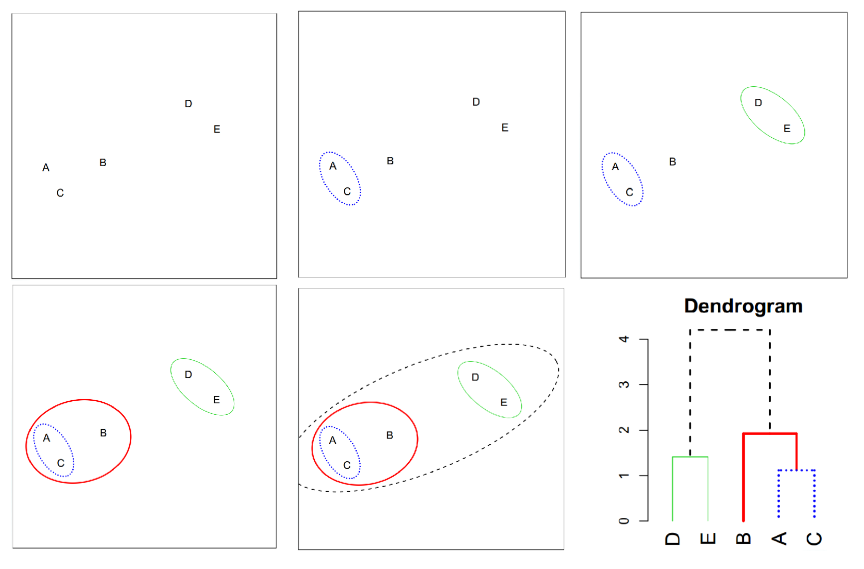
\includegraphics[width=0.7\linewidth]{sections/images/Hierarchical Clustering.png}
    \caption{Illustration of Hierarchical Clustering}
    \label{}
\end{figure}


\subsubsection{$ K $-Means Clustering Algorithm}
    \index{Clustering Analysis!$ K $-Means Clustering Algorithm}\index{k-Means Clustering Algorithm@$ k $-Means Clustering Algorithm}
    Assume we have a preset number $ K $ of clusters , we can use $ K $-means clustering.
\begin{algorithm}{$ K $-Means Clustering}
    \begin{enumerate}[topsep=2pt,itemsep=2pt]
        \item Choose/Preset number of clusters $ K $;
        \item Select $ K $ points as initial centroids, useful methods:
        \begin{itemize}[topsep=2pt,itemsep=2pt]
            \item Randomly select;
            \item Use Centroid of agglomerative algorithm;
            \item Successively pick the farthest point from others. 
        \end{itemize}
        \item In each iteration of centroids:
        \begin{enumerate}[topsep=2pt,itemsep=2pt]
            \item For all points $ i $, calculate its distance from the $ l^\mathrm{th} $ centroid $ D(i,l) $
            \item Classify each $ i $ point to the nearest centroid cluster;
            \item Re-calculate the centroid of new $ K $ clusters;
        \end{enumerate}
        \item Repeat until convergence.(Convergence criterion can be e.g. $ <\sum_i D(i\in g_l,l)>\to \mathrm{const} $)
    \end{enumerate}
\end{algorithm}
    





Note: pros­and­cons of $ K $-Means clustering algorithm
\begin{itemize}[topsep=2pt,itemsep=2pt]
    \item Efficient:$ \sim O(n) $;
    \item Sensitive to outliers;
    \item Ineffective for non-convex shapes.
\end{itemize}

    


\subsubsection{Expectation Maximization Algorithm for Gaussian Mixture Model}\label{SubSubSectionEMAlgorithmForGMM}
\index{Clustering Analysis!Expectation Maximization Algorithm}
\index{E-M Algorithm (Expectation Maximization Algorithm)}
    % We can also label each object, then conduct discriminant analysis (e.g. QDA).

    %  Assumption and notation:  
    % \begin{align*}
    %     Y\sim& \sum_{l=1}^k\pi_lN()\text{ where }\pi\text{ is a set }\{\pi_l\}\\
    %     X|Y=l\sim& N(\mu_l,\Sigma _l)=N(\theta_l),\, 1\leq l\leq k
    % \end{align*}

    % Our aim is to estimate $ \pi,(\mu_i,\Sigma _i) ,\,1\leq i\leq k$. 
    % Take two-component gaussion mixture model $ k=2 $ as example.
        The Gaussian Mixture Model (GMM)\index{GMM (Gaussian Mixture Model)} for clustering assumes $ X $ is generated from a mixed distribution of $ K $ normal, i.e. $ X $ has probability $ \pi_l $ to be generated from corresponding normal $ N(\mu _l,\Sigma _l) $:
    \begin{equation}
        X\sim \sum_{l=1}^K\pi_lN(\mu_l,\Sigma _l)=\sum_{l=1}^K\pi_lN(\theta _l),\quad \sum_{l=1}^K\pi_l=1,\,\pi_l\geq 0.
    \end{equation}
    
    Use its likelihood function $ L(\theta;x) $ and maximize posterior probability by $ \dfrac{\partial^{} \ell}{\partial \theta ^{}} $:
    \begin{equation}
        L(\{\pi_l\},\{\theta_l \};x)=\prod_{i=1}^N \sum_{l=1}^K\pi_l   \dfrac{1}{(2\pi)^{p/2}|\Sigma _l|^{1/2}}\exp\left(   -\dfrac{1}{2}(x_i-\mu _l)'\Sigma^{-1} _l(x_i-\mu _l)\right)
    \end{equation}
    
    E-M Algorithm uses the ELBO maximizing method, detail see \autoref{SubSectionExpectationMaximumAlgorithm}. For simplification express $ \theta \equiv \{ \cup \pi_l,\cup \mu_l,\cup \Sigma _l \} $. The maximizing function $ Q(\theta |\theta ^{(t)}) $ for GMM model and corresponding iteration: 
\begin{align*}
    \theta ^{(t+1)}=\mathop{\arg\max}\limits_{\theta }  Q(\theta |\theta ^{(t)})=&\mathop{\arg\max}\limits_{\theta }\sum_{i=1}^N\sum_{l=1}^K\gamma _{il}^{(t)}\log \pi_l\phi (x_i|\mu _l,\Sigma _l),\quad \gamma _{il}^{(t)}\equiv \dfrac{\pi_l^{(t)}\phi(x_i|\mu _l^{(t)},\Sigma _l^{(t)})}{\sum\limits_{j=1}^K\pi_j^{(t)}\phi (x_i|\mu _j^{(t)},\Sigma _j^{(t)})}
\end{align*}
    Lagrange Multiplier: Extreme value $ \mathop{\arg\max}\limits_{\theta }Q(\theta |\theta ^{(t)})  $ with constraint $ \sum_{l=1}^K \pi_l=1 $ requires 
    \begin{equation}
         \dfrac{\partial^{}  Q(\theta |\theta ^{(t)})}{\partial \mu _l^{}}=0\quad \dfrac{\partial^{}  Q(\theta |\theta ^{(t)})}{\partial \Sigma ^{-1}_l}=0 \quad \dfrac{\partial^{}  Q(\theta |\theta ^{(t)})+\lambda (\sum_{j=1}^K\pi_l-1)}{\partial \pi_j^{}}=0,\quad \forall l=1,2,\ldots,K
    \end{equation}
    
    Result:
    \begin{align}\label{EqaGMMEMIteration}
        % &\sum_{i=1}^N\dfrac{\pi_l\phi _{\theta_l}(x_i)}{\sum\limits_{j=1}^k\pi_j\phi _{\theta_j}(x_i)}
        \begin{cases}
        \mu _l^{(t+1)}=&\dfrac{\sum\limits_{i=1}^N\gamma _{il}^{(t)}x_i}{\sum\limits_{i=1}^N\gamma^{(t)}_{il}}\\
        \Sigma _l^{(t+1)}=&\dfrac{\sum\limits_{i=1}^N\gamma^{(t)} _{il}(x_i-\mu _l)(x_i-\mu _l)'}{\sum\limits_{i=1}^N\gamma ^{(t)}_{il}}\\
        \pi_l^{(t+1)}=&\dfrac{1}{N}\sum_{i=1}^N\gamma^{(t)}_{il}
        \end{cases}
    \end{align}
\begin{equation}
        \gamma ^{(t)}_{il}\equiv \dfrac{\pi_l^{(t)}\phi(x_i|\mu _l^{(t)},\Sigma _l^{(t)})}{\sum\limits_{j=1}^K\pi_j^{(t)}\phi (x_i|\mu _j^{(t)},\Sigma _j^{(t)})} 
\end{equation}  
    
    
    
    where $ \gamma _{il} $ is the posterior probability that the $ i^\mathrm{th} $ object belongs to the $ l^\mathrm{th} $ group.

    The above constraint equations are difficult to solve, use iteration algorithm:
\begin{algorithm}{EM-Algorithm for Gaussian Mixture Model}
    \begin{enumerate}[topsep=2pt,itemsep=2pt]
        \item Use e.g. $ K $-means method to set an initial estimation as $ (\hat{\mu}^{(0)}_l,\hat{\Sigma }_l^{(0)}),\,\hat{\pi}_l^{(0)}=1/K$;
        \item Repeat Expectation \& Maximization:
        \begin{enumerate}[topsep=2pt,itemsep=2pt]
            \item $ \mathrm{E_{xpectation}} $-Step: Compute posterior of latent variable on each point;
        \begin{equation}
            \hat{\gamma }_{il}^{(t)}=\dfrac{\pi_l^{(t)}\phi(x_i|\mu _l^{(t)},\Sigma _l^{(t)})}{\sum\limits_{j=1}^K\pi_j^{(t)}\phi (x_i|\mu _j^{(t)},\Sigma _j^{(t)})} ,\quad  1\leq i\leq N,\,\, 1\leq l\leq K
        \end{equation}
        \item $ \mathrm{M_{aximize}} $-Step: Re-calculate parameters $ \{\mu_l,\Sigma _l,\pi_l\} $ by \autoref{EqaGMMEMIteration}.
        \end{enumerate}
        \item Repeat until convergence.
    \end{enumerate}
\end{algorithm}
    
    Note: EM method for Gaussion Mixture Model is a greedy algorithm $ \longrightarrow $ local maximum.
    
\subsubsection{DBSCAN \& OPTICS Density Clustering Algorithm}
    \index{Clustering Analysis!Density Clustering}
    \hyperlink{DBSCAN}{DBSCAN} algorithm (Density-Based Spatial Clustering of Application with Noise)\index{Clustering Analysis!DBSCAN (Density-Based Spatial Clustering of Application with Noise)} is a kind of density clustering algorithm. \hyperlink{OPTICS}{OPTICS} algorithm (Ordering Point To Indentify the Cluster Structure) is its improved version.


\begin{point}
    \hypertarget{DBSCAN}{DBSCAN} Algorithm
\end{point}

    Key (preset) index in DBSCAN:
    \begin{itemize}[topsep=2pt,itemsep=2pt]
        \item Eps $ \varepsilon  $: Radius of neighbourhood of a point;
        \item MinPts $ M $: Minimum number of points to be indentified as cluster core point, usually choose $ M\geq \mathrm{dim}+1 $;
        \item (Also, a distance norm is needed, e.g. Euclidean $ D $).
    \end{itemize}
    
    Notation:
    \begin{itemize}[topsep=2pt,itemsep=2pt]
        \item $ \varepsilon  $ neighbourhood of point $ x_i $:
        \begin{equation}
             \mathcal{N}_\varepsilon (x_i)\equiv \{y\in \mathbb{R} ^n: 0<D(y,x)<\varepsilon \}
        \end{equation}
        \item `Density' (is actually an integer):
        \begin{equation}
            \rho _\varepsilon (x_i)\equiv \#  x_j\in \mathcal{N}_\varepsilon (x_i) 
        \end{equation}
        \item Three types of Points: $ X_c $, $ X_{bd} $, $ X_{noi} $.
        \begin{itemize}[topsep=2pt,itemsep=2pt]
            \item Core Point: label an $ x_i $ as core point if
        \begin{equation}
            \rho _\varepsilon (x_i)\geq M
        \end{equation}

        Denote the set of core point as $ X_c $, and set of non-core point as $ X_{nc} $
        
        \item Border Point: label an $ x_j\in X_{nc} $ as border point if
        \begin{equation}
             \exists (x_i\in X_c)\in \mathcal{N}_\varepsilon (x_j) \& x_j\in X_{nc}
        \end{equation}
        Denote the set of border point as $ X_{bd} $
        \item Noise Point: the set of noise point is 
        \begin{equation}X_{noi}\equiv\displaystyle{\complement_X^{X_{c}\cup X_{bd}} }\end{equation}
        \end{itemize}
    \item Point Relations: DDR, DR, DC
    \begin{itemize}[topsep=2pt,itemsep=2pt]
    \item Directly Density Reachable: For $ x_i,x_j\in X $, if $ x_i\in X_c $, $ x_j\in\mathcal{N}_\varepsilon (x_i) $, then say $ x_j $ is DDR from $ x_i $;
    \item Density Reachable: For point chain $ x_{i_1},x_{i_2},\ldots,x_{i_m} $, $ m\geq 2 $. If $ x_{i_{\kappa+1} } $ is DDR from $ x_{i_\kappa } $, $ \forall 1\leq \kappa \leq m-1 $, then say $ x_{i_m} $ is DR from $ x_{i_1} $.
    \item Density Connected: For point $ x_{i_1} $, $ x_{i_2} $, $ x_{i_3} $, if $ x_{i_2} $ and $ x_{i_3} $ are both DR from $ x_{i_1} $, then say $ x_{i_2} $ and $ x_{i_3} $ are DC. 
    \end{itemize}
    
    Note: DR is not symmetric for $ x_{i_1} $ and $ x_{i_m} $; while DC is.       
    \end{itemize}
    
    DBSCAN algorithm classify all points that are Density Connected to each other into a cluster $ C\subset X $, i.e.
    \begin{align*}
        \text{Maximality:}& x\in C\&\& y\text{ DR from } x \Rightarrow y\in C\\
        \text{Connectivity:}& x,y\in C\Rightarrow x,y\text{ DC}.
    \end{align*} 
        
    Pros and cons of DBSCAN:
\begin{itemize}[topsep=2pt,itemsep=2pt]
    \item Insensitive to noise;
    \item Based on density, with no constraint on the shape of cluster; 
    \item Suitable for clusters with uniformly densed data, otherwise difficult to choose proper Eps $ \varepsilon  $;
    \item Complexity $ \sim O(n^2) $, at least $ O(n\log n) $.
\end{itemize}


\begin{point}
    \hypertarget{OPTICS}{OPTICS} Algorithm\index{Clustering Analysis!OPTICS (Ordering Point To Indentify the Cluster Structure)}
\end{point}

    OPTICS is based on DBSCAN and shares most of the basic concepts and ideas. Further define the following distance (preset $ \varepsilon  $ and $ M $):
    \begin{itemize}[topsep=2pt,itemsep=2pt]
        \item Core Distance: For $ x_i\in X_c $, the smallest distance allowing $ x_i $ to become core point.
        \begin{equation}
            \mathrm{CD}(x_i)=D(x_i,N^M_\varepsilon (x_i)),\, \rho _\varepsilon (x_i)\geq M
        \end{equation}

        where $ N^M_\varepsilon (x_i) $ is the $ M^\mathrm{th} $ closest point from $ x_i $;
        \item Reachablity Distance: For $ y\in X,\,x_i \in X_c\subset X$, 
        \begin{equation}
            \mathrm{RD}(y,x_i)=\max\{CD(x_i,D(y,x_i))\}
        \end{equation}

        Or equivlantly
        \begin{equation}
            \mathrm{RD}(y,x_i)=\mathop{\arg\min}\limits_{\rho _d(x_i)\geq M, y\in \mathcal{N}_d(x_i)}  d
        \end{equation}
        
        
    \end{itemize}
    
        
    Algorithm flow:
\begin{algorithm}{OPTICS }

\begin{enumerate}[topsep=2pt,itemsep=2pt]
    \item Construct $ X_c $ based on preset $ M $, $ \varepsilon  $;
    % \item Denoting two sequence: \lstinline|Order seq| and \lstinline|Outcome seq|;
    \item Pick an `unprocessed' point $ x_{n_i}\in X_c $ and calculate $ \mathrm{RD}(x_j,x_{n_i} ) $, $ \forall \text{`unprocessed'} x_j\in \mathcal{N}_\varepsilon (x_{n_i}) \cap X_c $. Pick the $ x_j\in X_c $ with smallest RD and label as $ x_{n_{i+1}} $ processed;
    \item Repeat step 2 until all points are processed. Output $ \{x_{n_i}\}=(x_{n_1},x_{n_2},\ldots,x_{n_{|X_c|}}) $. Each $ x_{n_i} $ is attached with a $ \mathrm{CD}(x_{n_i}) $ and a $ r(x_{n_i}):=\mathrm{RD}(x_{n_{i-1}},x_{n_i}) $\footnote{For $ i=1 $, just define as $ 0 $}.
\end{enumerate}
    
\end{algorithm}
    

    Then break the ordering sequence $ n_i $ according to $ r(x_{n_i}) $, .e.g. break $ n_i $ if $ r(x_{n_i})\geq \tilde{\varepsilon } $

    Comment: OPTICS is more stable than DBSCAN, capable of dealing with multi-density clustering.





